\documentclass[10pt,a4paper]{article}
\usepackage{amsmath}
\usepackage{amsfonts}
\usepackage{amssymb}
\usepackage[english]{babel}
\usepackage{float}
\usepackage[left=2cm,right=2cm,top=2cm,bottom=2cm]{geometry}
\usepackage{graphicx}
\usepackage{hyperref} % Used for external links
\usepackage[utf8]{inputenc}
\usepackage{listings} % Used for source code listing

% Source code listing's parameters
\lstset{
  frame=single,
  keepspaces=true,
%  title=\lstname
}

\title{First SPICE Exercise\\{\small{Fundamentals Of Electronics - a.a. 2018-2019 -
University of Padua (Italy)}}}
\author{Pietro Prandini (mat. 1097752)}

\begin{document}
\maketitle

% License
\begin{center}
\tiny{This work is licensed under the Creative Commons Attribution-ShareAlike
 4.0 International License. To view a copy of this license, visit
 \href{http://creativecommons.org/licenses/by-sa/4.0/}{http://creativecommons.org/licenses/by-sa/4.0/}
or send a letter to Creative Commons, PO Box 1866, Mountain View, CA 94042,
USA.}
\end{center}

\section{Audio amplifier}
\subsection{Voltage gain and frequency domain - Ideal op. amp.}
\begin{figure}[h]
  \centering
  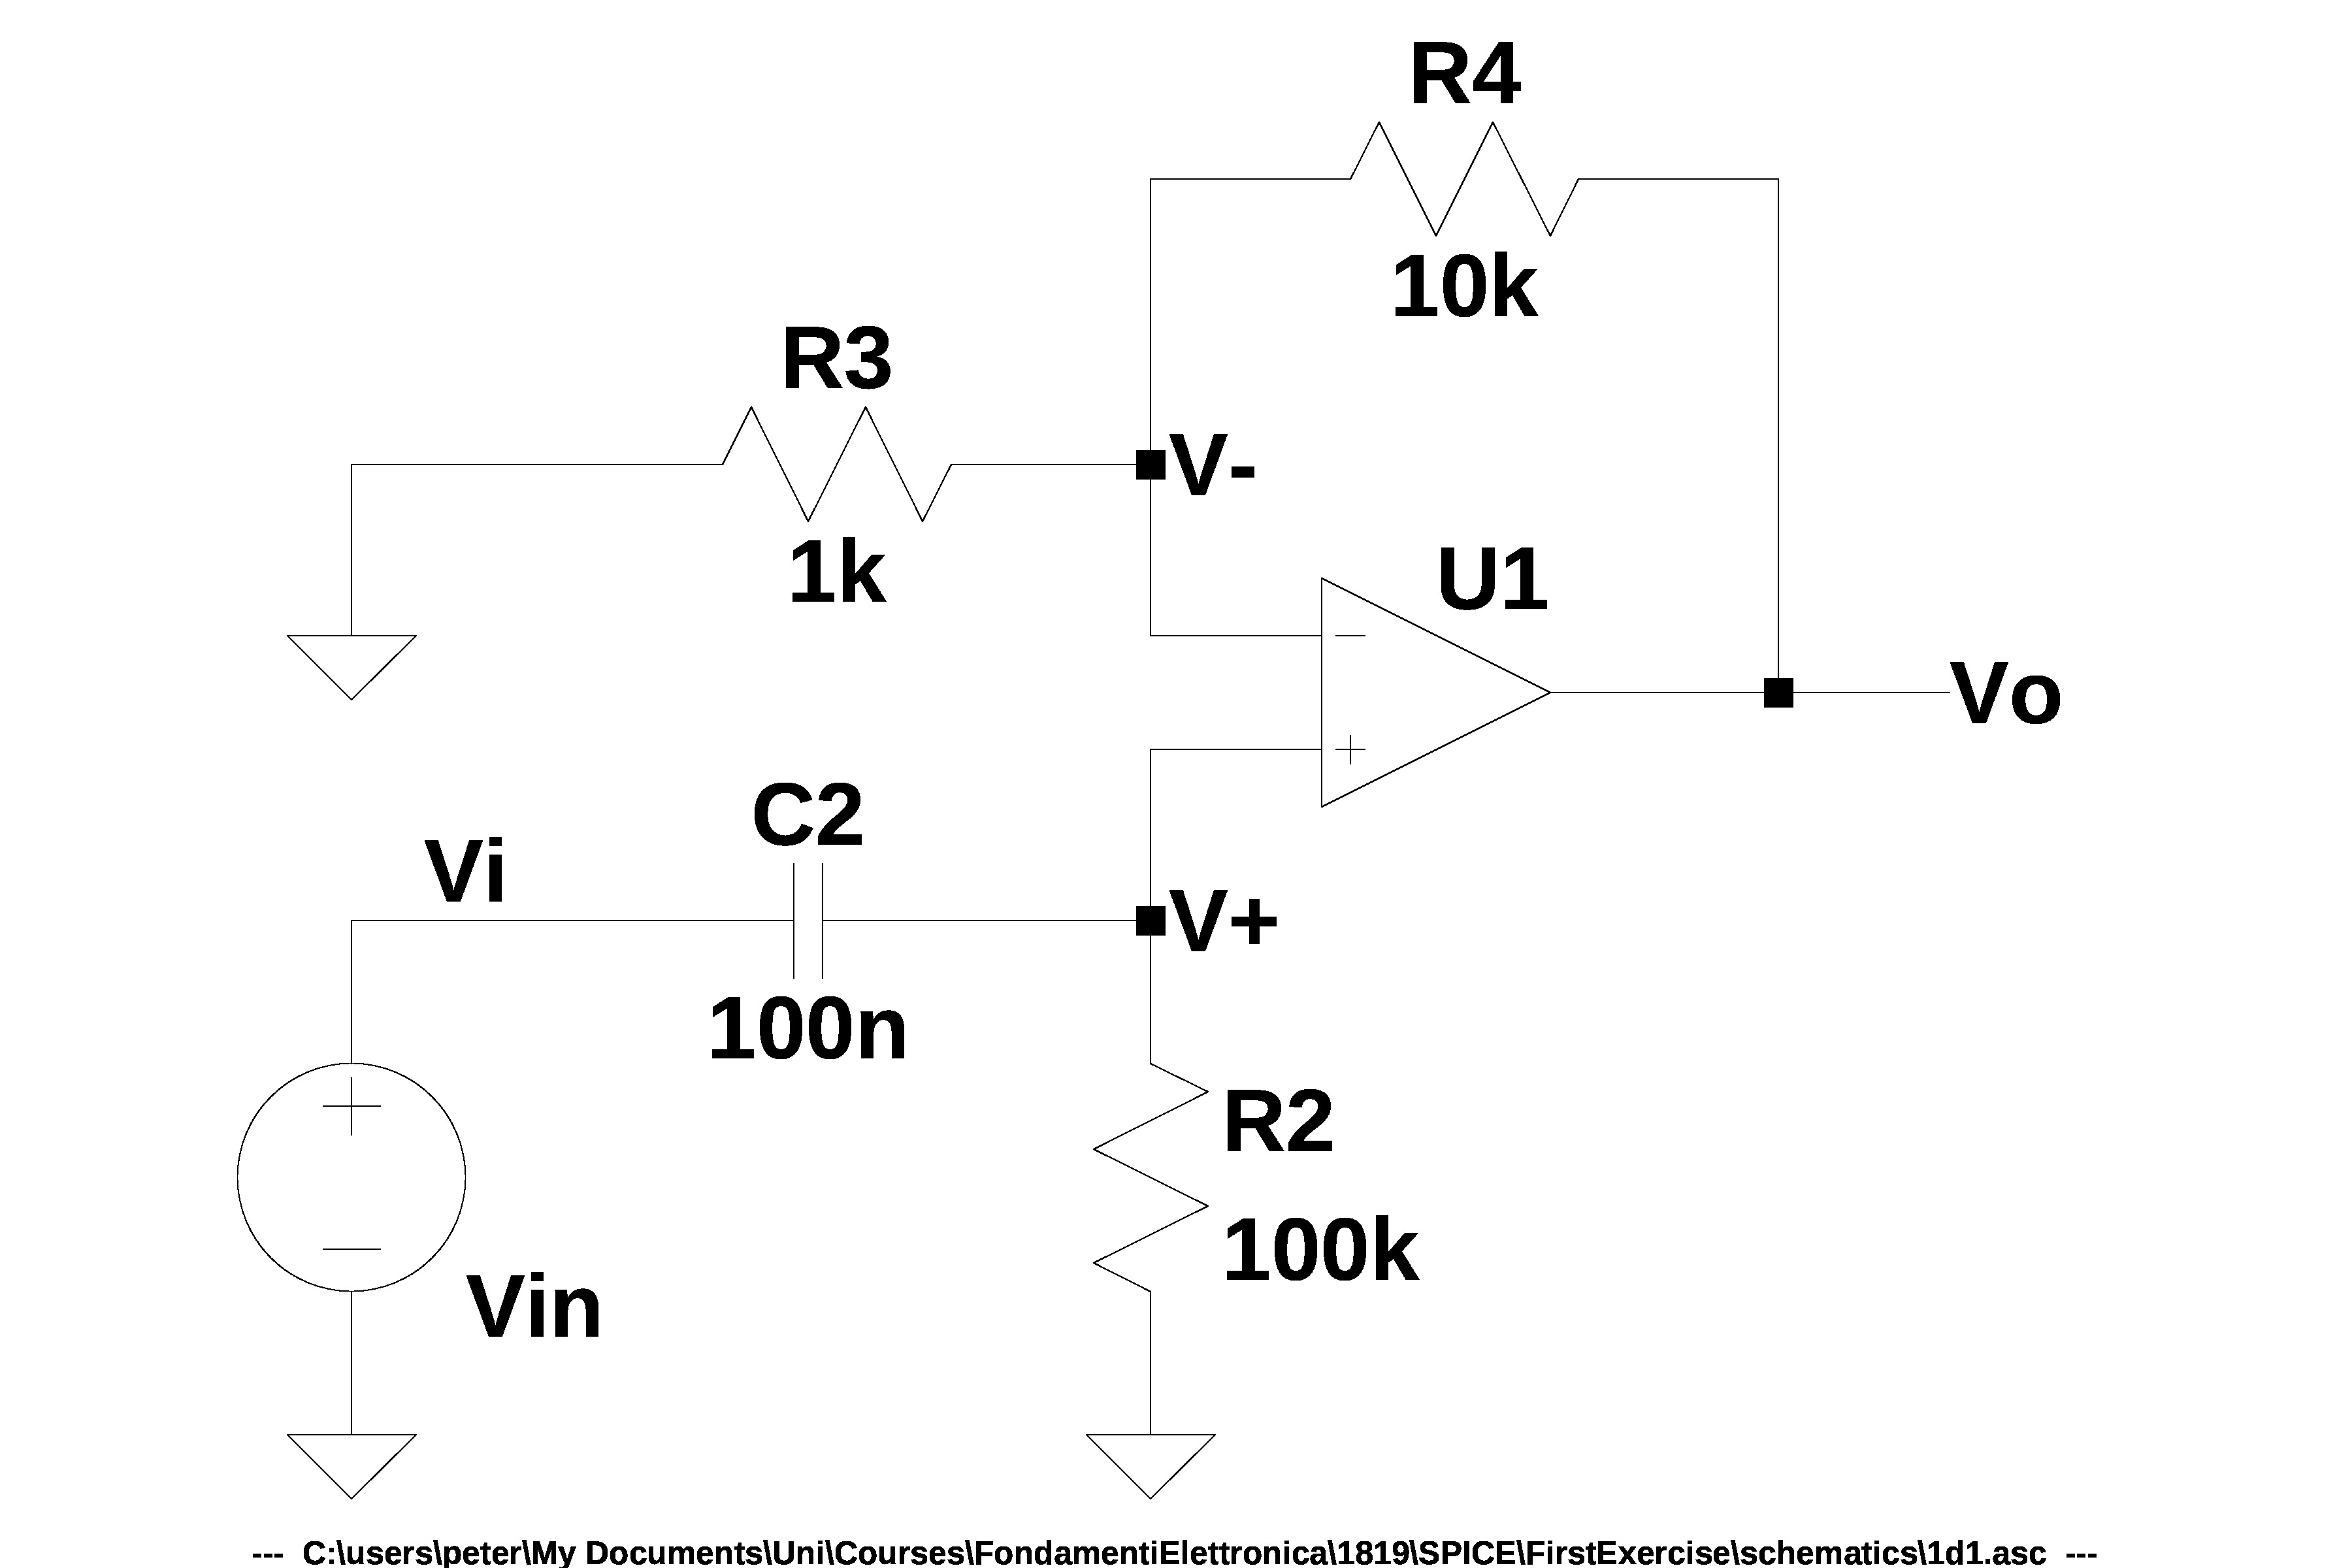
\includegraphics[width=8cm]{schematics/1d1.jpg}
  \caption{Audio amplifier - Ideal op. amp.}
  \label{1d1schematics}
\end{figure}

By the analysis of the figure \ref{1d1schematics}'s circuit, It's possible to
calculate the node $V_+$ voltage from the ratio of the voltage divider formed by
$R_2$ and $C_2$, infact the node $V_+$ voltage is the same voltage of the
resistance $R_2$ (equation \ref{eq:V_+}).\\
\begin{equation} \label{eq:V_+}
V_+(s) = V_{in}(s)\frac{R_2}{R_2+\frac{1}{sC_2}} =
V_{in}(s)\frac{R_2}{R_2+\frac{1}{sC_2}}\frac{sC_2}{sC_2} =
V_{in}(s)\frac{sC_2R_2}{1+sC_2R_2}
\end{equation}

The negative feedback produces the virtual short circuit effect, so the $V_-$
and the $V_+$ voltages have virtually the same value (equation \ref{eq:V_-}),
and, because of the fact that the ideal operational amplifier $U_1$ isn't
absorbe current from the $V_-$ and the $V_+$ nodes, the current of $I_{R_4}$ is
the same current of $I_{R_3}$ (equation \ref{eq:I_R4}).\\
The current $I_{R_3}$ is calculated by the Ohm law (equation \ref{eq:I_R3}).\\
\begin{equation} \label{eq:V_-}
V_- = V_+
\end{equation}

\begin{equation} \label{eq:I_R4}
I_{R_4} = I_{R_3}
\end{equation}

\begin{equation} \label{eq:I_R3}
I_{R_3} = \frac{V_-}{R_3} = \frac{V_+}{R_3}
\end{equation}

By combining the past considerations it's possible to define the output voltage
$V_o$ relating to the voltage input $V_{in}$ (equation \ref{eq:V_o}).\\
\begin{equation} \label{eq:V_o}
V_o(s) = V_+(s) + R_4I_{R_4} = V_+(s) + R_4 I_{R_3} = V_+(s) + R_4 \cdot \frac{V_+(s)}{R_3} =
V_+(s) \cdot \left(1 + \frac{R_4}{R_3} \right) =
V_{in}(s)\frac{sC_2R_2}{1+sC_2R_2} \cdot \left(1 + \frac{R_4}{R_3} \right)
\end{equation}

Conseguently of the equation \ref{eq:V_o}, the transfer funtion
$V_o(s)/V_{in}(s)$ is descripted by the equation \ref{eq:TF}.\\
\begin{equation} \label{eq:TF}
\frac{V_o(s)}{V_{in}(s)} = \frac{sC_2R_2}{1+sC_2R_2}\left(1+\frac{R_4}{R_3}\right)
\end{equation}

Defining $K$ as in the equation \ref{eq:K} and $\omega_1$ as in the equation \ref{eq:omega_1}, the transfer function $V_o(s)/V_{in}(s)$ became in the Bode form (equation \ref{eq:TFBode}).\\
\begin{equation} \label{eq:K}
K = C_2R_2 \cdot \left(1+\frac{R_4}{R_3}\right)
\end{equation}

\begin{equation} \label{eq:omega_1}
 \omega_1 = \frac{1}{C_2R_2}
\end{equation}

\begin{equation} \label{eq:TFBode}
\frac{V_o(s)}{V_{in}(s)} = K \frac{s}{1+s\frac{1}{\omega_1}}
\end{equation}

Finally it's possible to calculate the frequency domain by the analysis of the transfer function's Bode form (equations \ref{eq:KdB} and \ref{eq:omega_1log}).\\
\begin{equation} \label{eq:KdB}
 K|_{dB} = 20\log_{10}|K| = \log_{10}\left|C_2R_2 \cdot \left(1+\frac{R_4}{R_3}\right)\right| = -19.1722 dB
\end{equation}

\begin{equation} \label{eq:omega_1log}
\log_{10} |\omega_1| =
\log_{10} \left| \frac{1}{C_2R_2} \right|= 2.0000
\end{equation}

\subsection{Voltage output waveform - LT1028 op. amp.}
\begin{figure}[h]
  \centering
  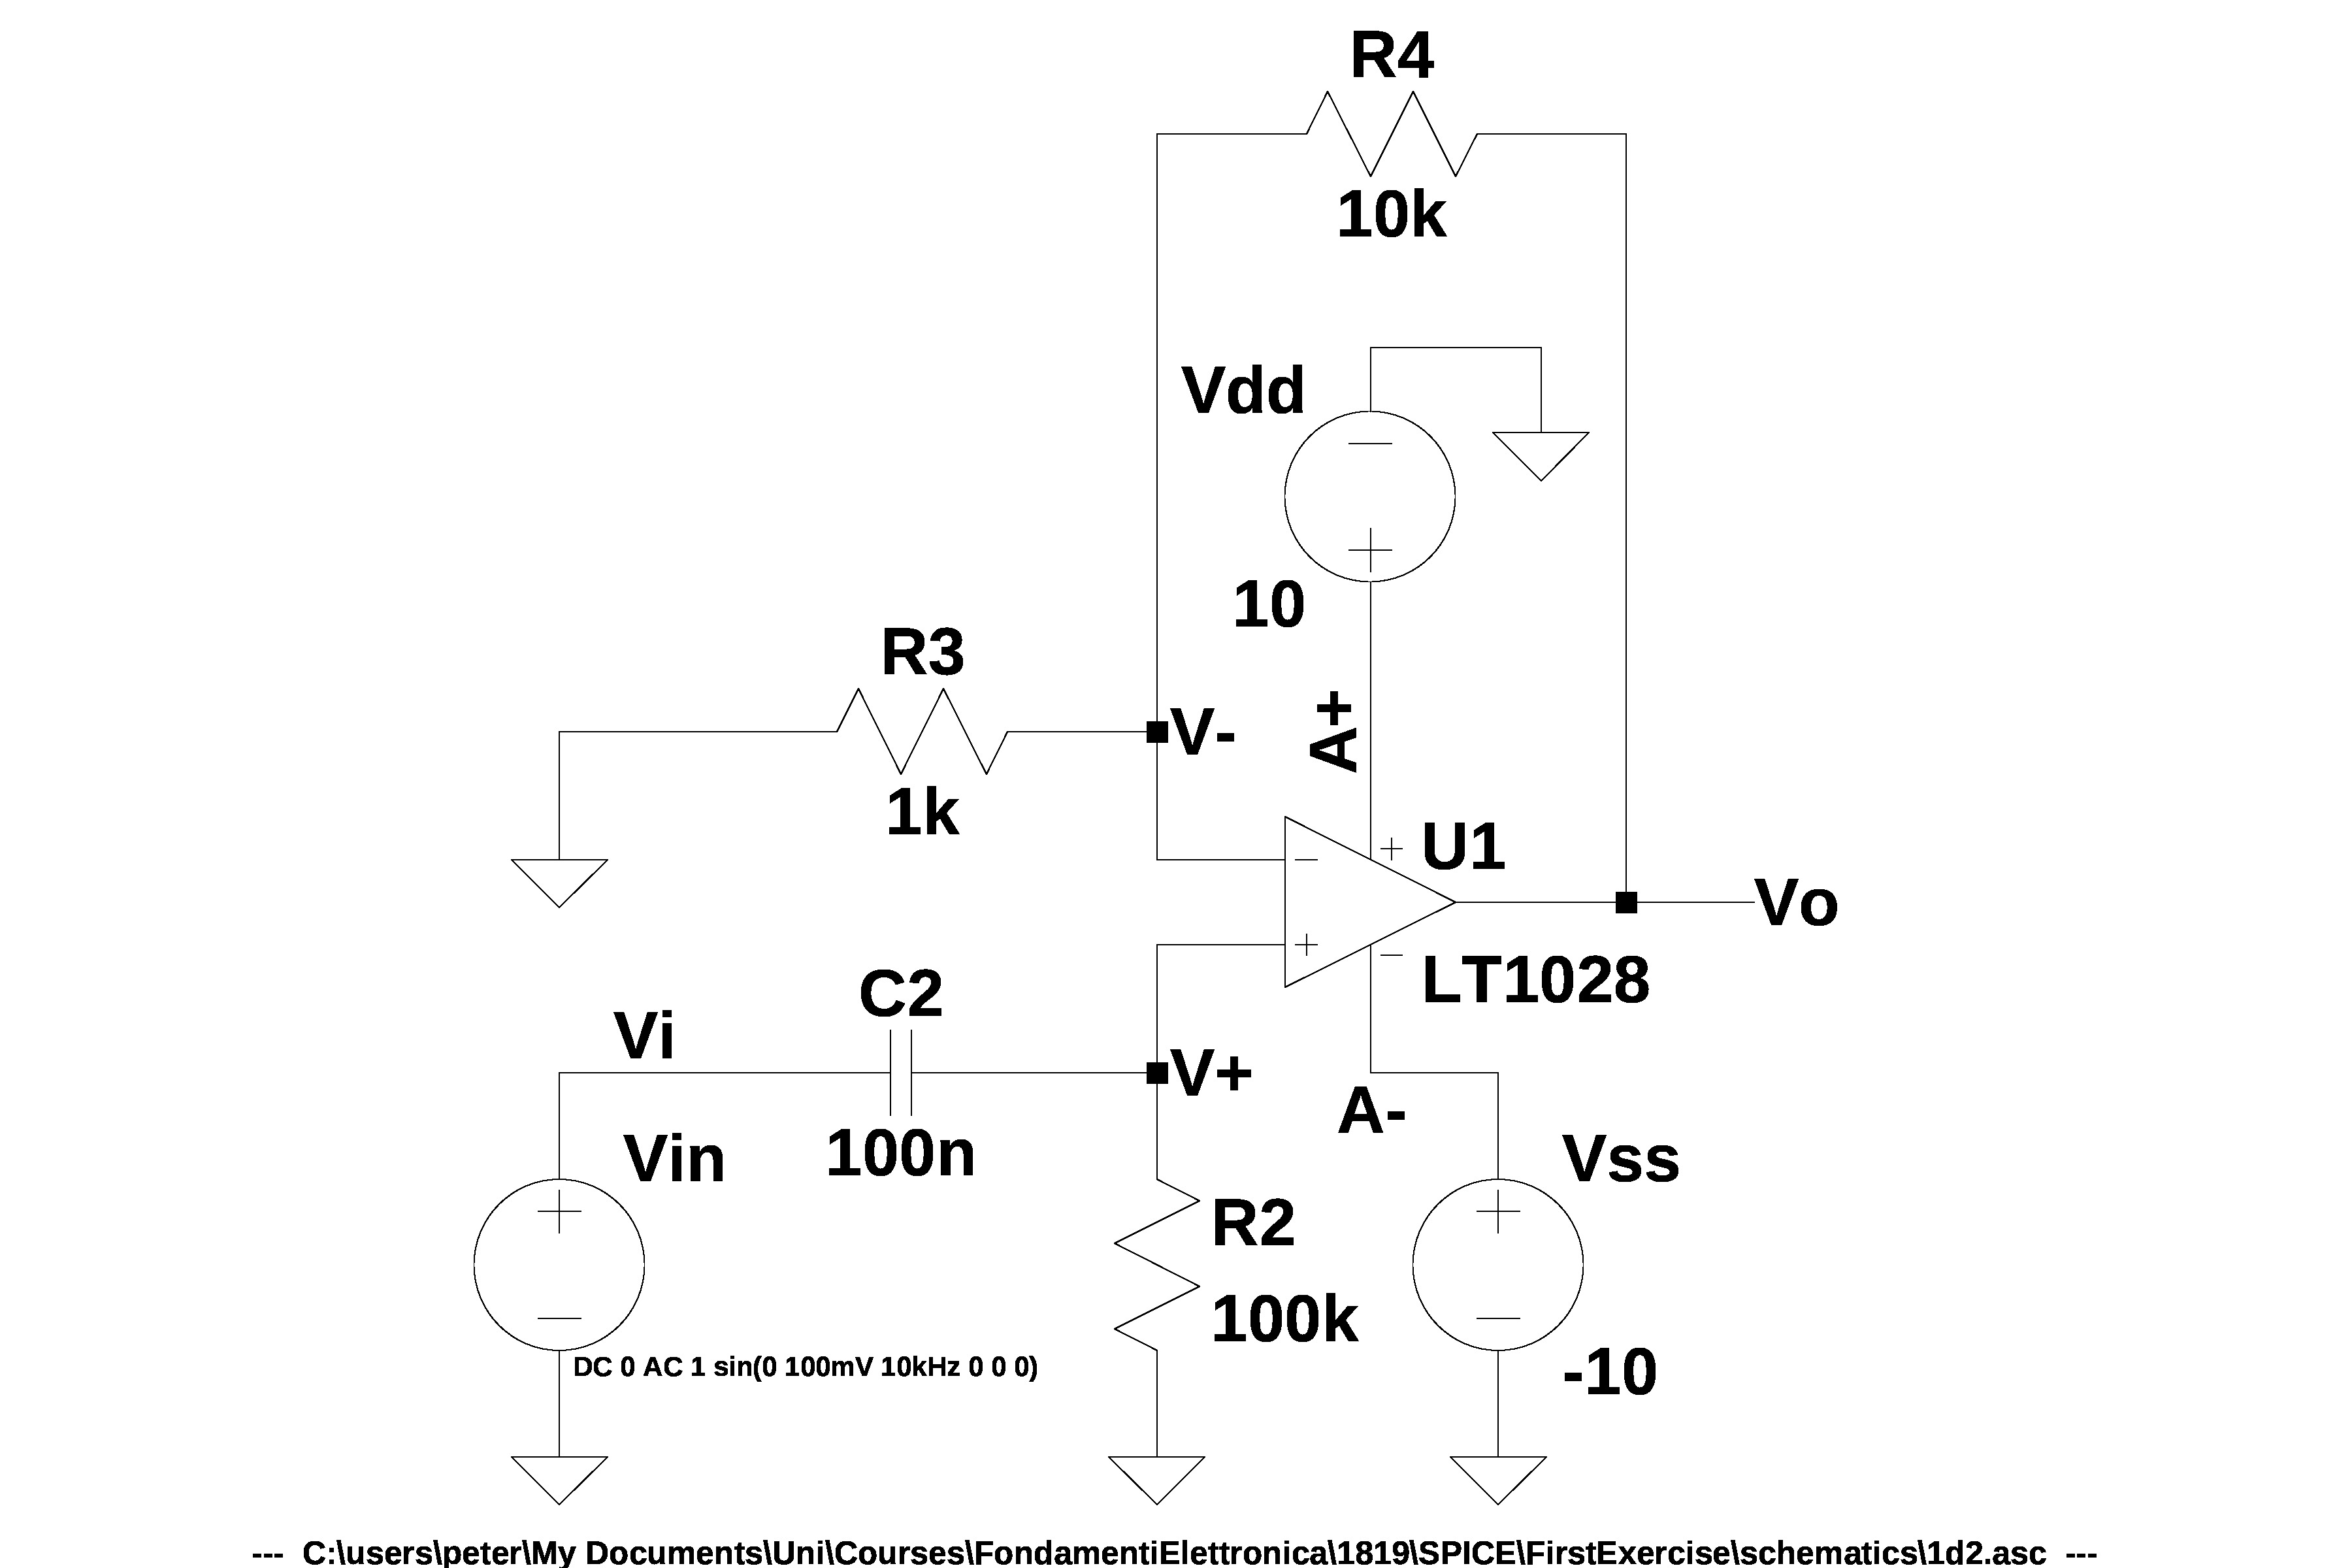
\includegraphics[width=10cm]{schematics/1d2.jpg}
  \caption{Audio amplifier - LT1028 op. amp.}
  \label{1d2schematics}
\end{figure}

From now it's considered the circuit of the figure \ref{1d2schematics}.\par
\medskip
In order to simulate the waveform output voltage with a sinusoidal voltage input $V_{in}$ with an amplitude of $10mV$ and the frequencies of $1Hz$, $10Hz$ and $10kHz$, it's possible to use a SPICE transient analysis.\\

\subsubsection{Netlist}
It's presented the netlist for the SPICE analysis requested.
\lstinputlisting{netlist/1d2.cir}

\subsubsection{Graph}
This graph is the output of the last netlist presented. There are three curves, one for every frequency analyzed ($1Hz$, $10Hz$ and $10kHz$).
\begin{figure}[H]
  \centering
  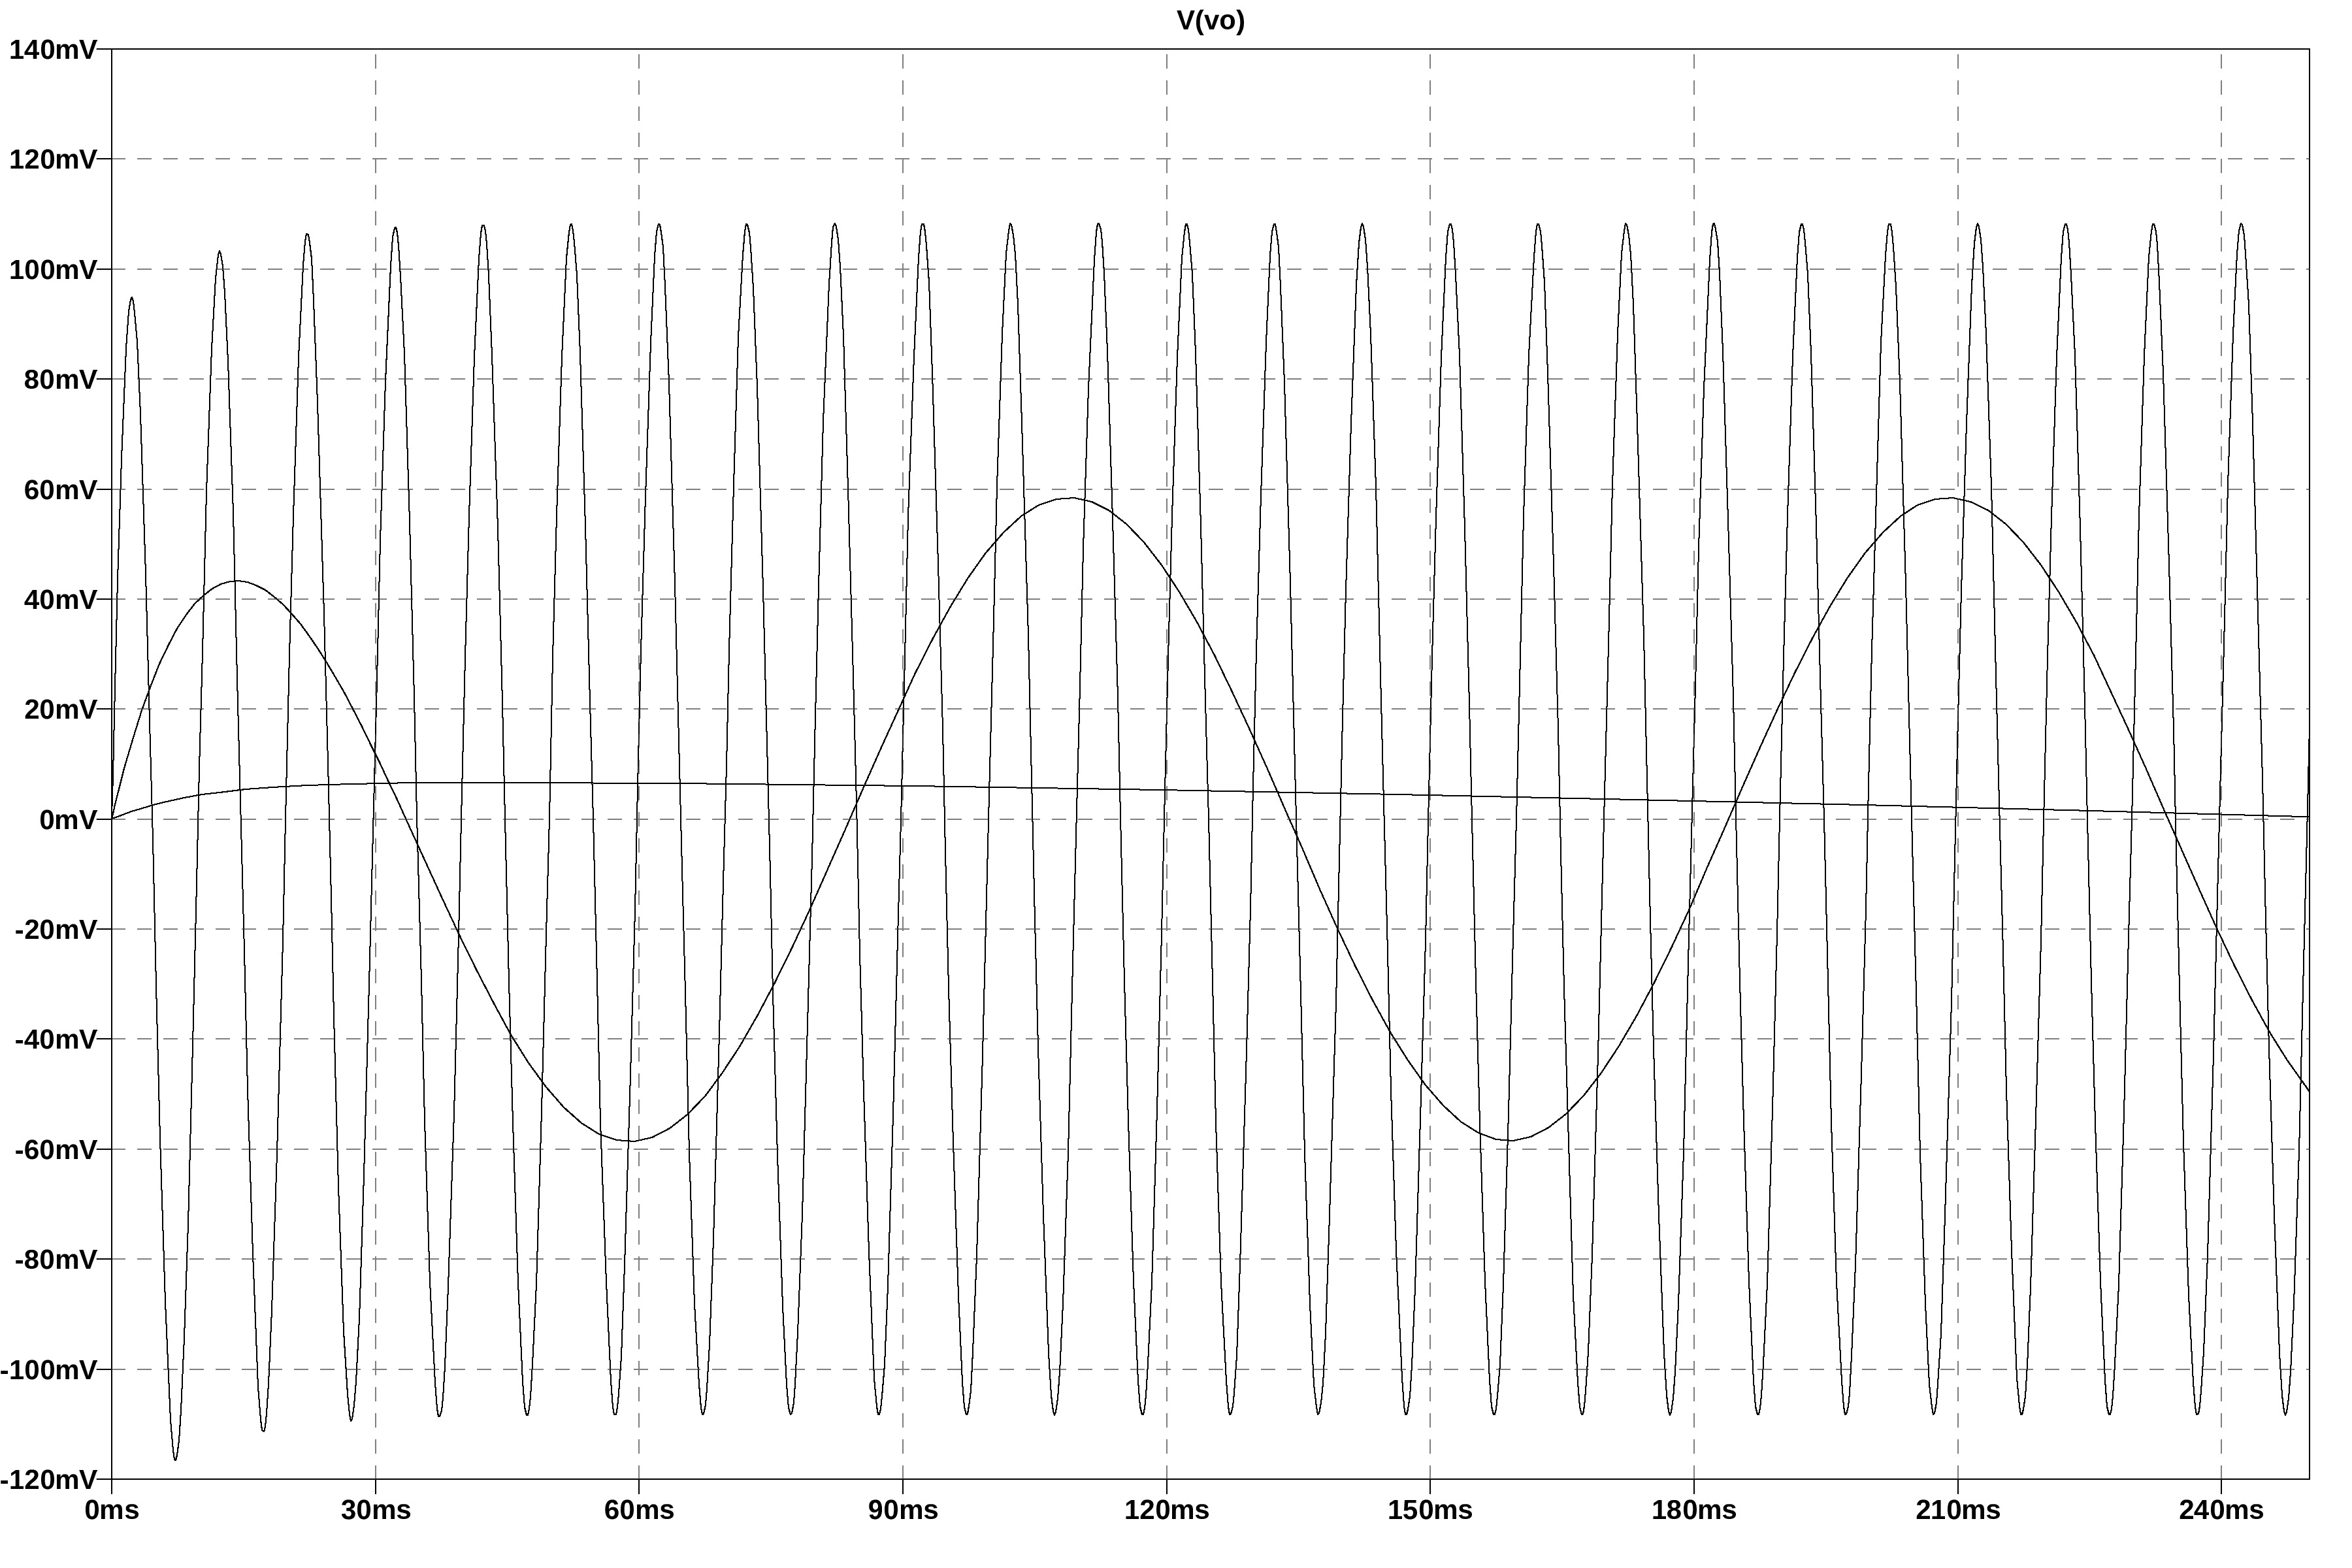
\includegraphics[width=14cm]{graph/1d2.jpg}
  \caption{Audio Amplifier - Voltage output waveform}
  \label{1d2graph}
\end{figure}

\subsection{Bode plot - LT1028 op. amp.}
The Bode plot could be generated with a SPICE small signal AC analysis.\par

\subsubsection{Netlist}
It's presented the netlist for the SPICE analysis requested.
\lstinputlisting{netlist/1d3.cir}

\subsubsection{Graph}
The Bode plot generated could be visible in the figure \ref{1d3graph}.
The continuous line represents the magnitude and the dashed line represents the phase frequency.\\
\begin{figure}[H]
  \centering
  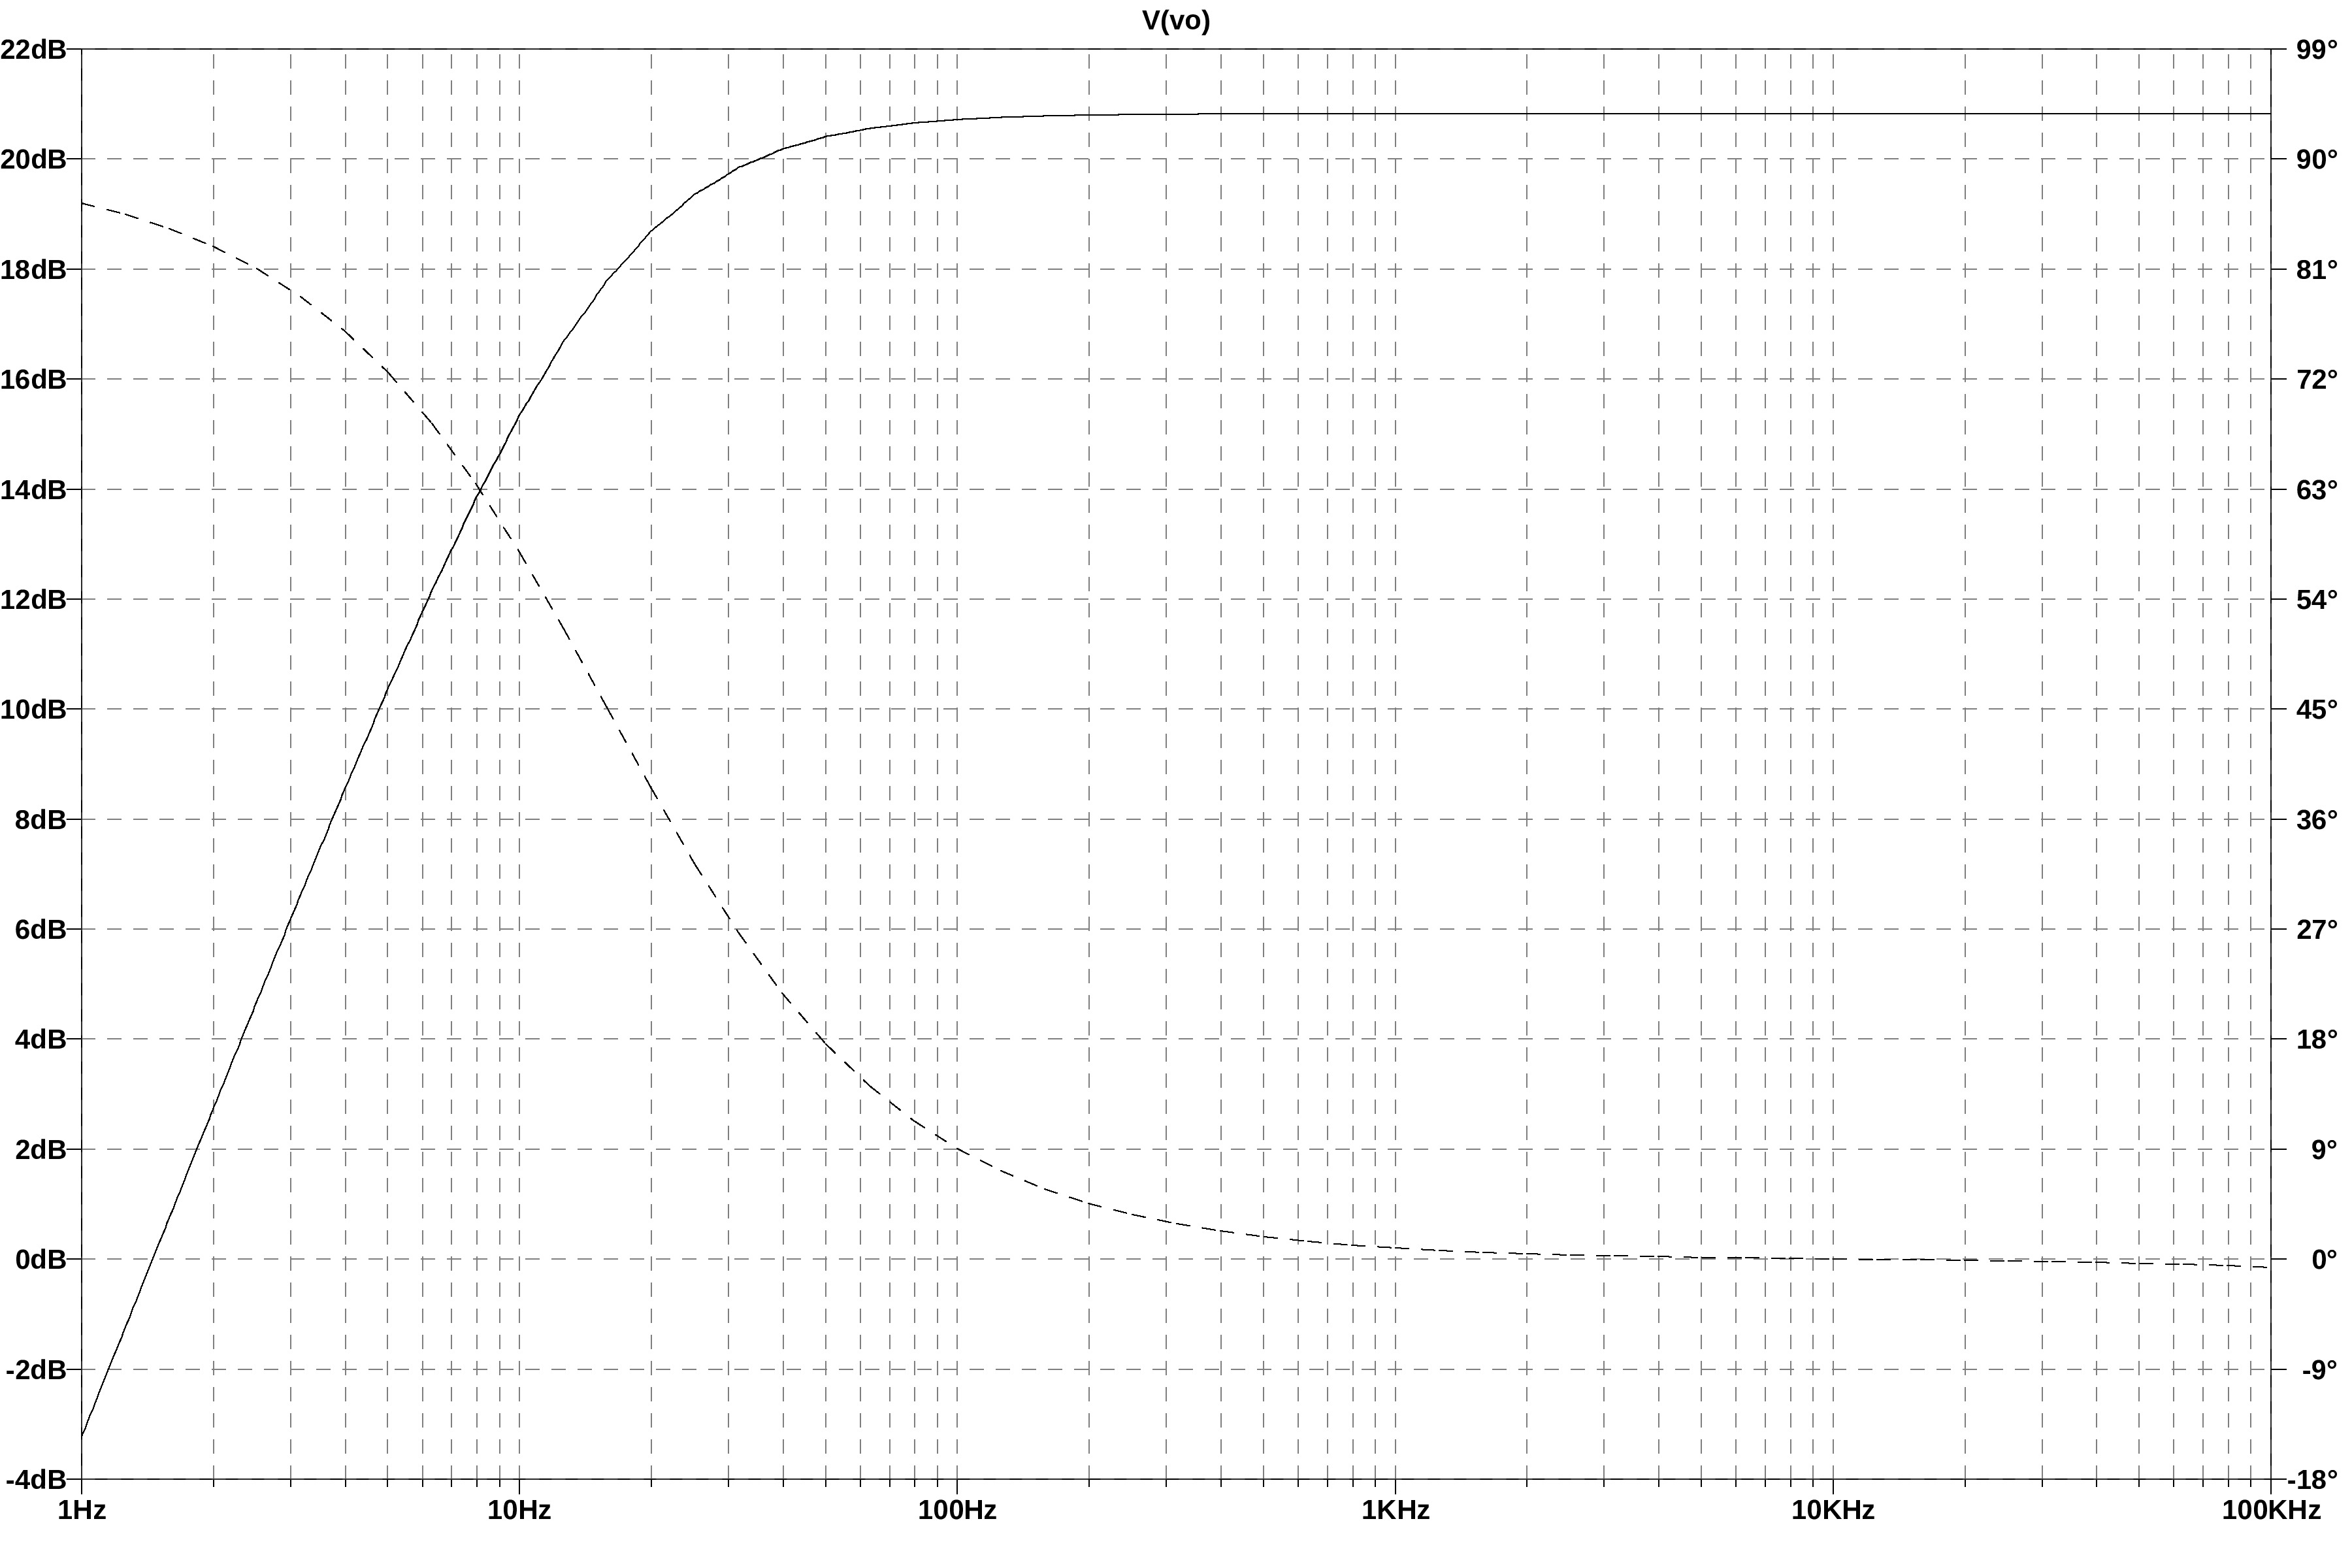
\includegraphics[width=14cm]{graph/1d3.jpg}
  \caption{Audio Amplifier - Bode plot}
  \label{1d3graph}
\end{figure}

\subsection{Saturation - LT1028 op. amp.}
The voltage output saturation could be analized by giving an abnormally high voltage input to the input.\\
The next netlist analyzes the voltage output with an input with $100V$ amplitude.\\

\lstinputlisting{netlist/1d4.cir}

\begin{figure}[H]
  \centering
  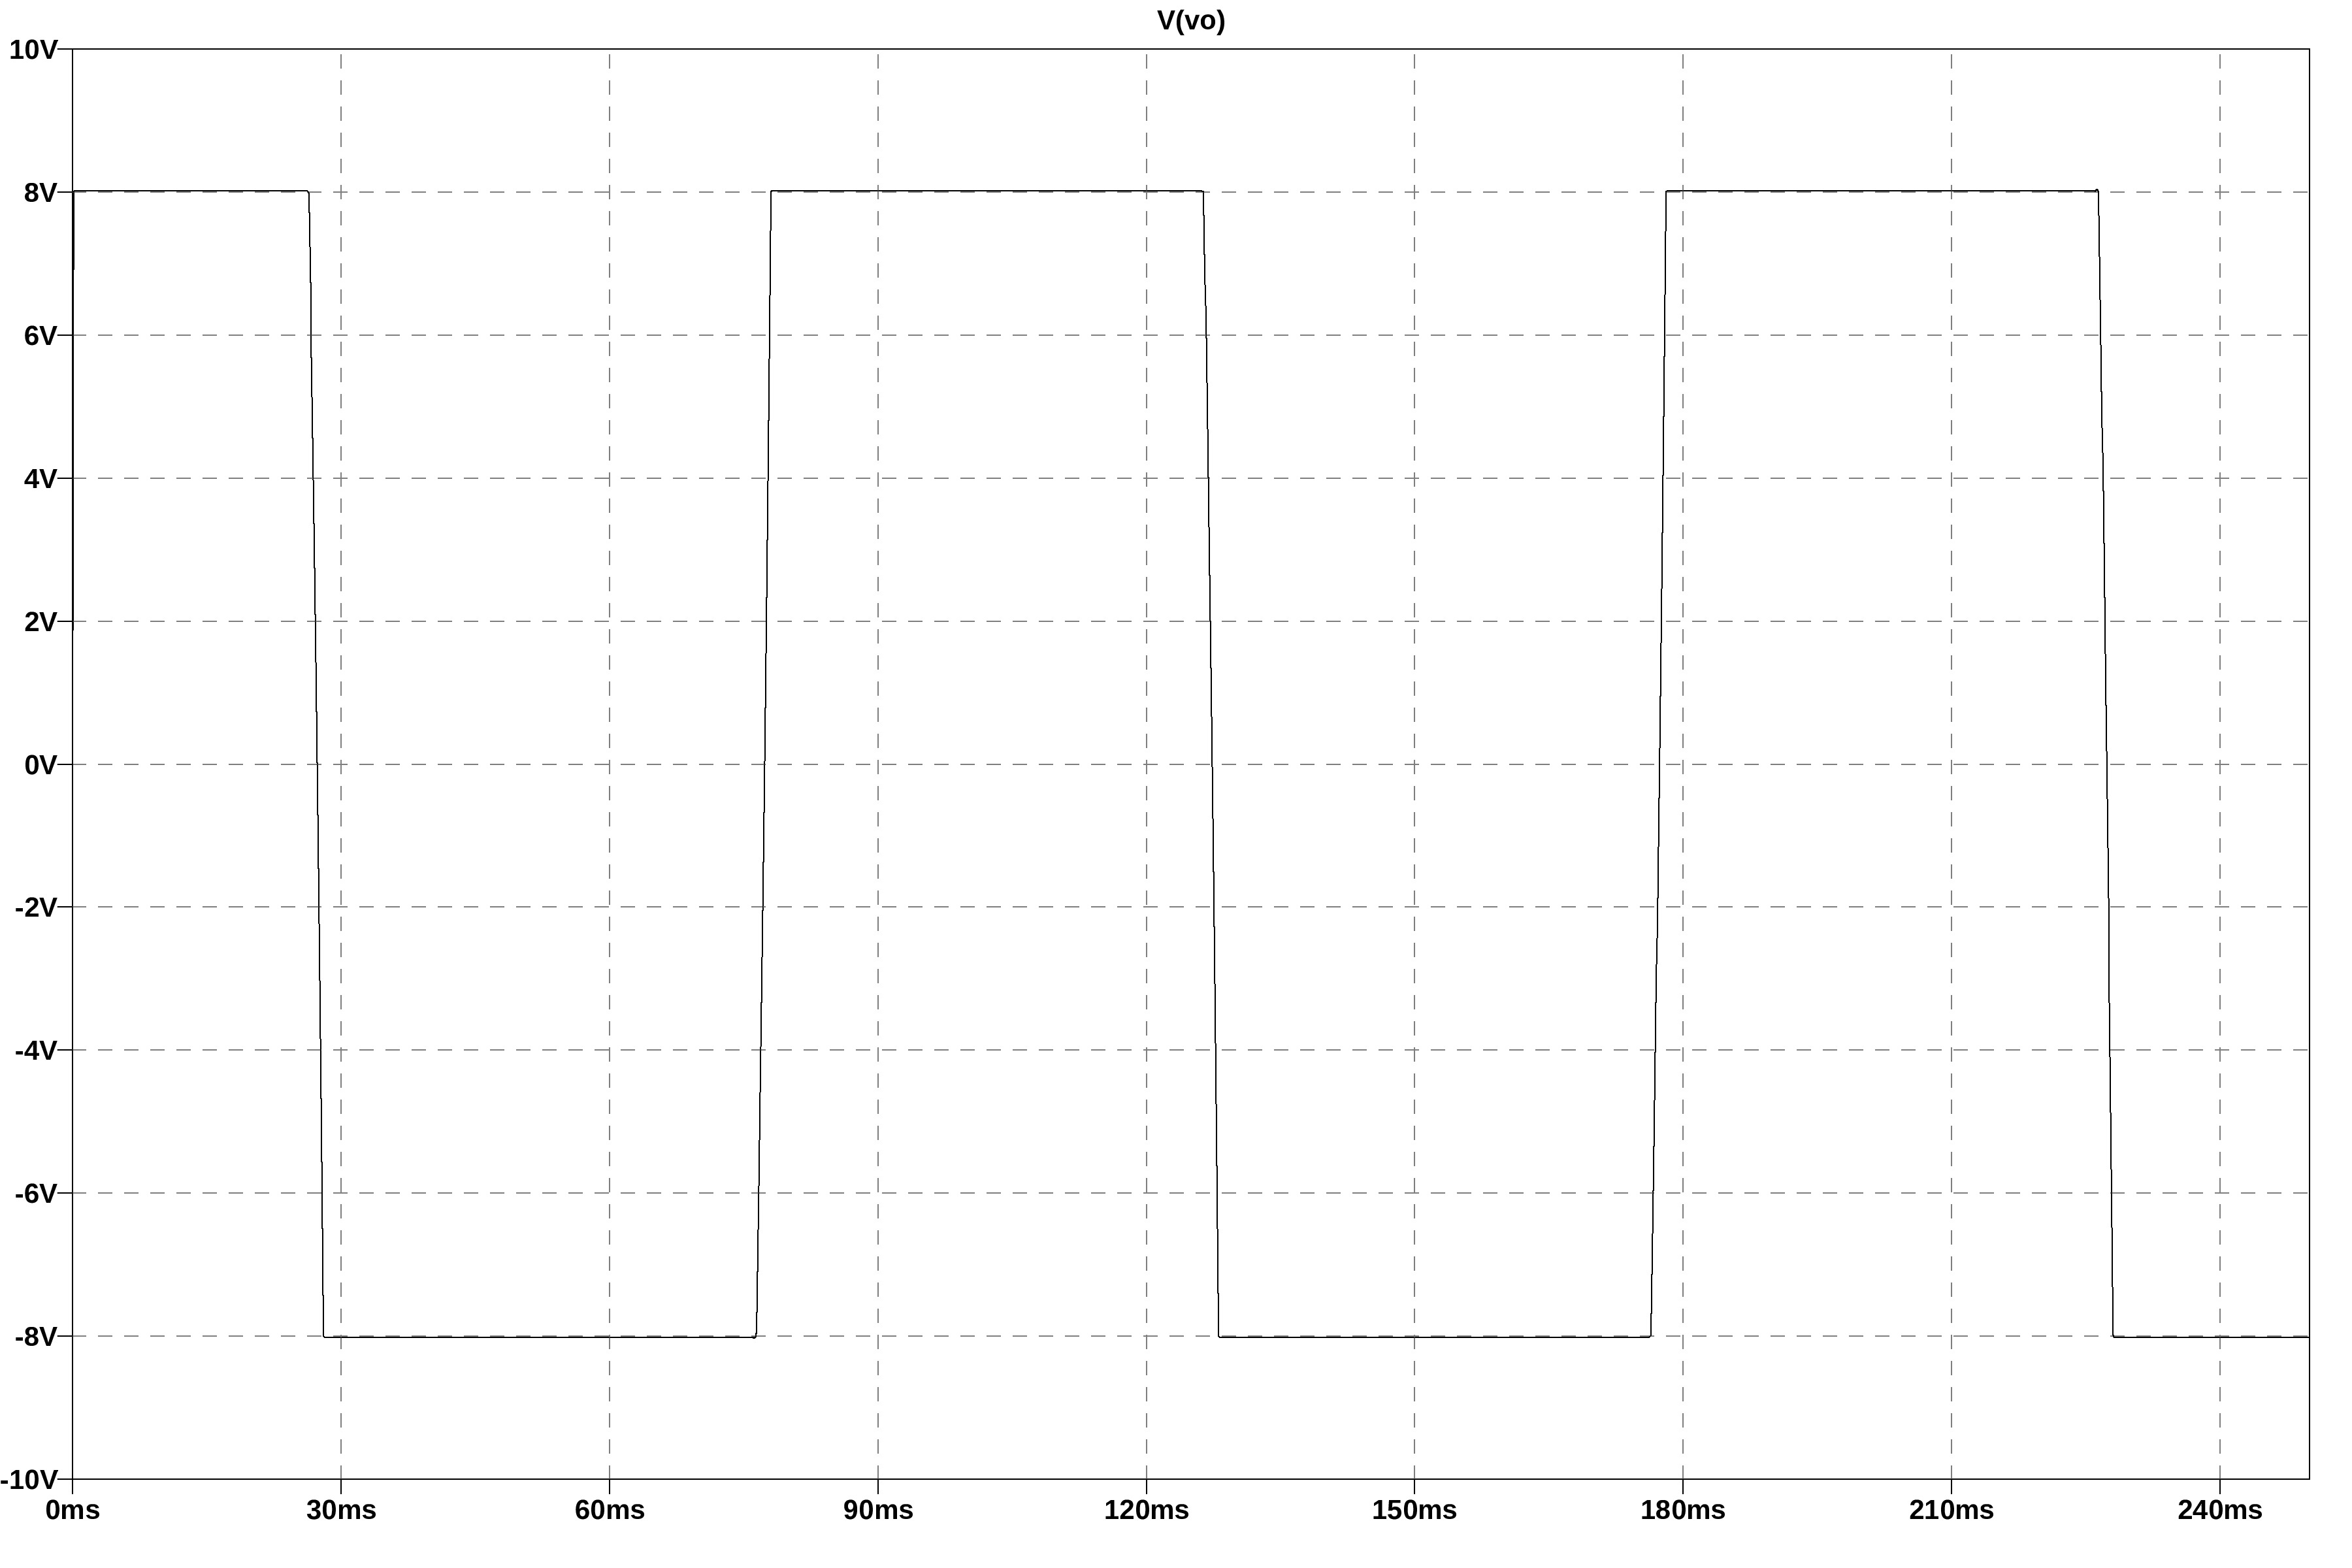
\includegraphics[width=14cm]{graph/1d4.jpg}
  \caption{Audio Amplifier - Output voltage saturation}
  \label{1d4graph}
\end{figure}
The graph generated (figure \ref{1d4graph}) makes clear the fact that the voltage output saturation is on $\pm8V$.\\
So it's possible to calculate wich is the highest input signal that avoids the saturation (equation \ref{eq:V_inSat}).\\

\begin{align}
|V_o| \leq 8V \nonumber \\
\left|V_{in}\cdot \frac{j\omega C_2R_2}{1+j\omega C_2R_2} \cdot \left(1 + \frac{R_4}{R_3} \right) \right| \leq 8V \nonumber \\
|V_{in}|\cdot \left|\frac{j\omega C_2R_2}{1+j\omega C_2R_2} \right| \cdot \left| \left(1 + \frac{R_4}{R_3} \right) \right| \leq 8V \nonumber \\
|V_{in}|\cdot \frac{\sqrt{(\omega C_2R_2)^2}}{\sqrt{1+(\omega C_2R_2)^2}} \cdot \frac{R_3 + R_4}{R_3} \leq 8V \nonumber \\
|V_{in}| \leq 8V \cdot \frac{\sqrt{1+(\omega C_2R_2)^2}}{\omega C_2R_2} \cdot \frac{R_3}{R_3 + R_4} \label{eq:V_inSat}
\end{align}

In order to have a maximum value of the input voltage $V_{in}$, the $\omega$ could be setted to a static value.\\
For example with $\omega = 10Hz \cdot 2\pi$ the maximum value of the input voltage is $|V_{in}| \leq 1.36701V$ (output voltage graph on figure \ref{1d4bgraph}).

\begin{figure}[H]
  \centering
  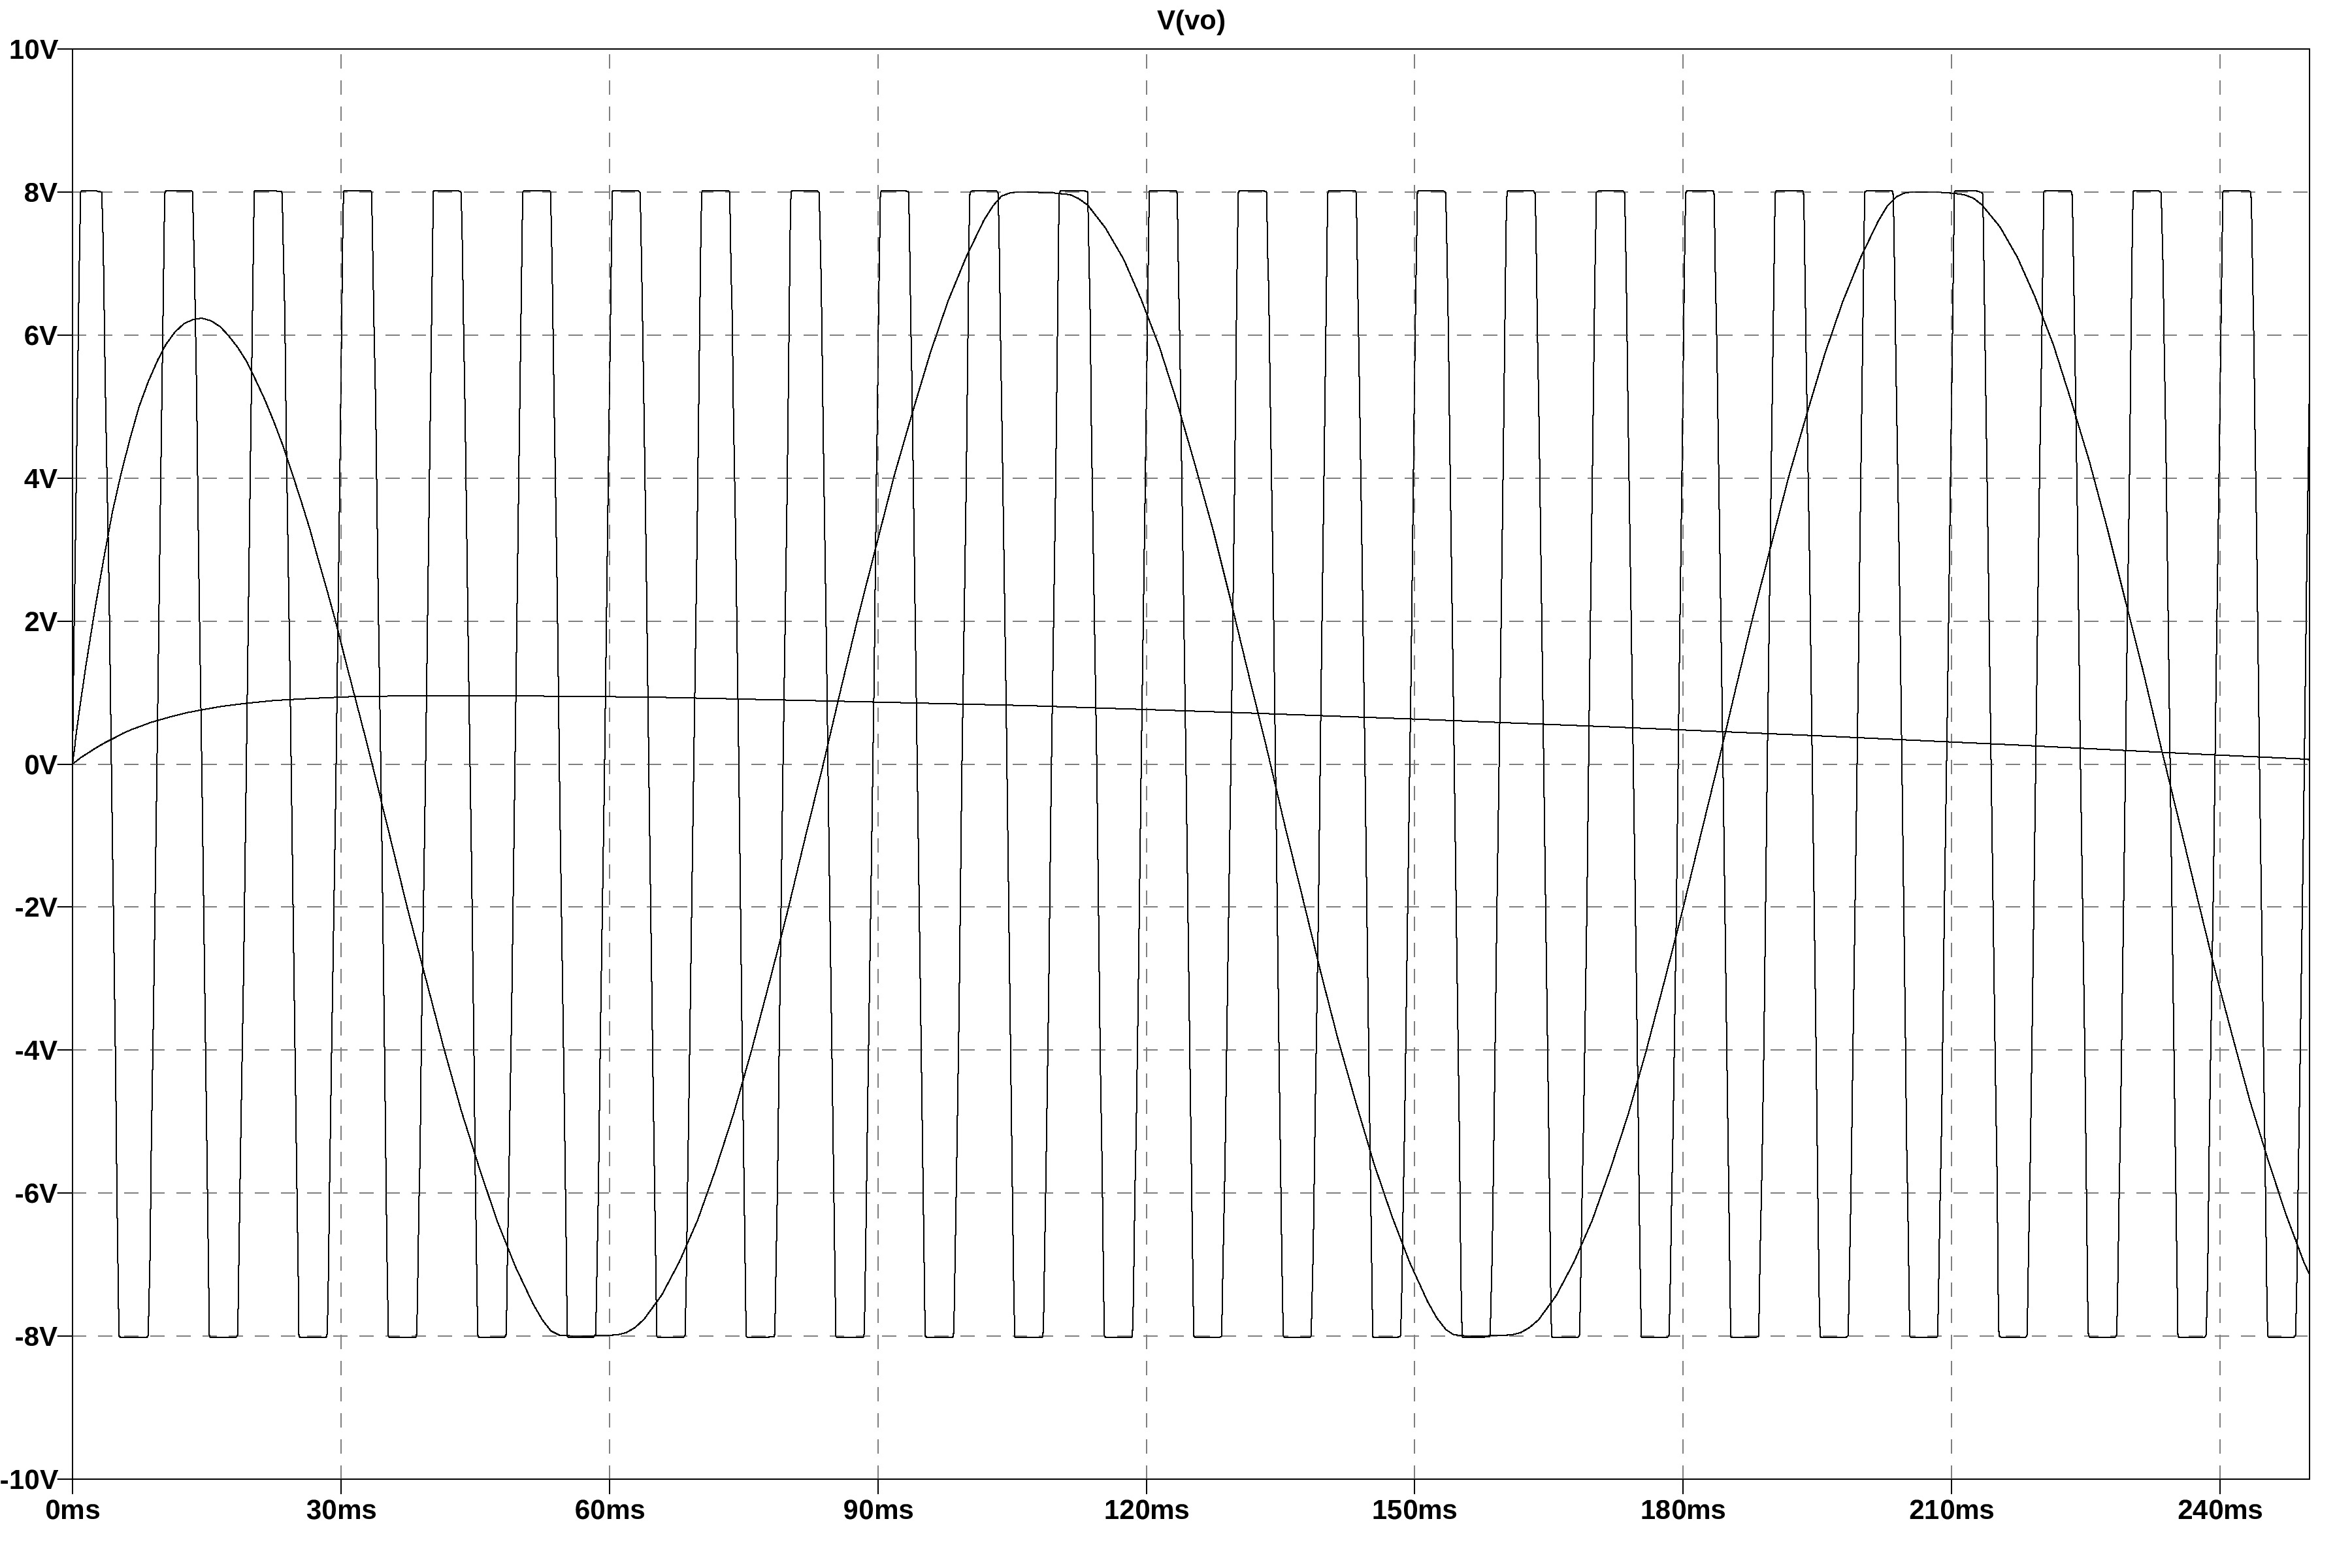
\includegraphics[width=14cm]{graph/1d4b.jpg}
  \caption{Audio Amplifier - Output voltage with an amplitude of the imput voltage equal to $1.36701V$, frequency equal to $10Hz$}
  \label{1d4bgraph}
\end{figure}

\subsubsection{Output voltage waveform - $V_{in} = 2 \cdot |V_{in MAX} |$}
The netlist used for plot the output voltage waveform with a double input voltage relatively to the maximum input voltage calculated is:\\
\lstinputlisting{netlist/1d4c.cir}

\begin{figure}[H]
  \centering
  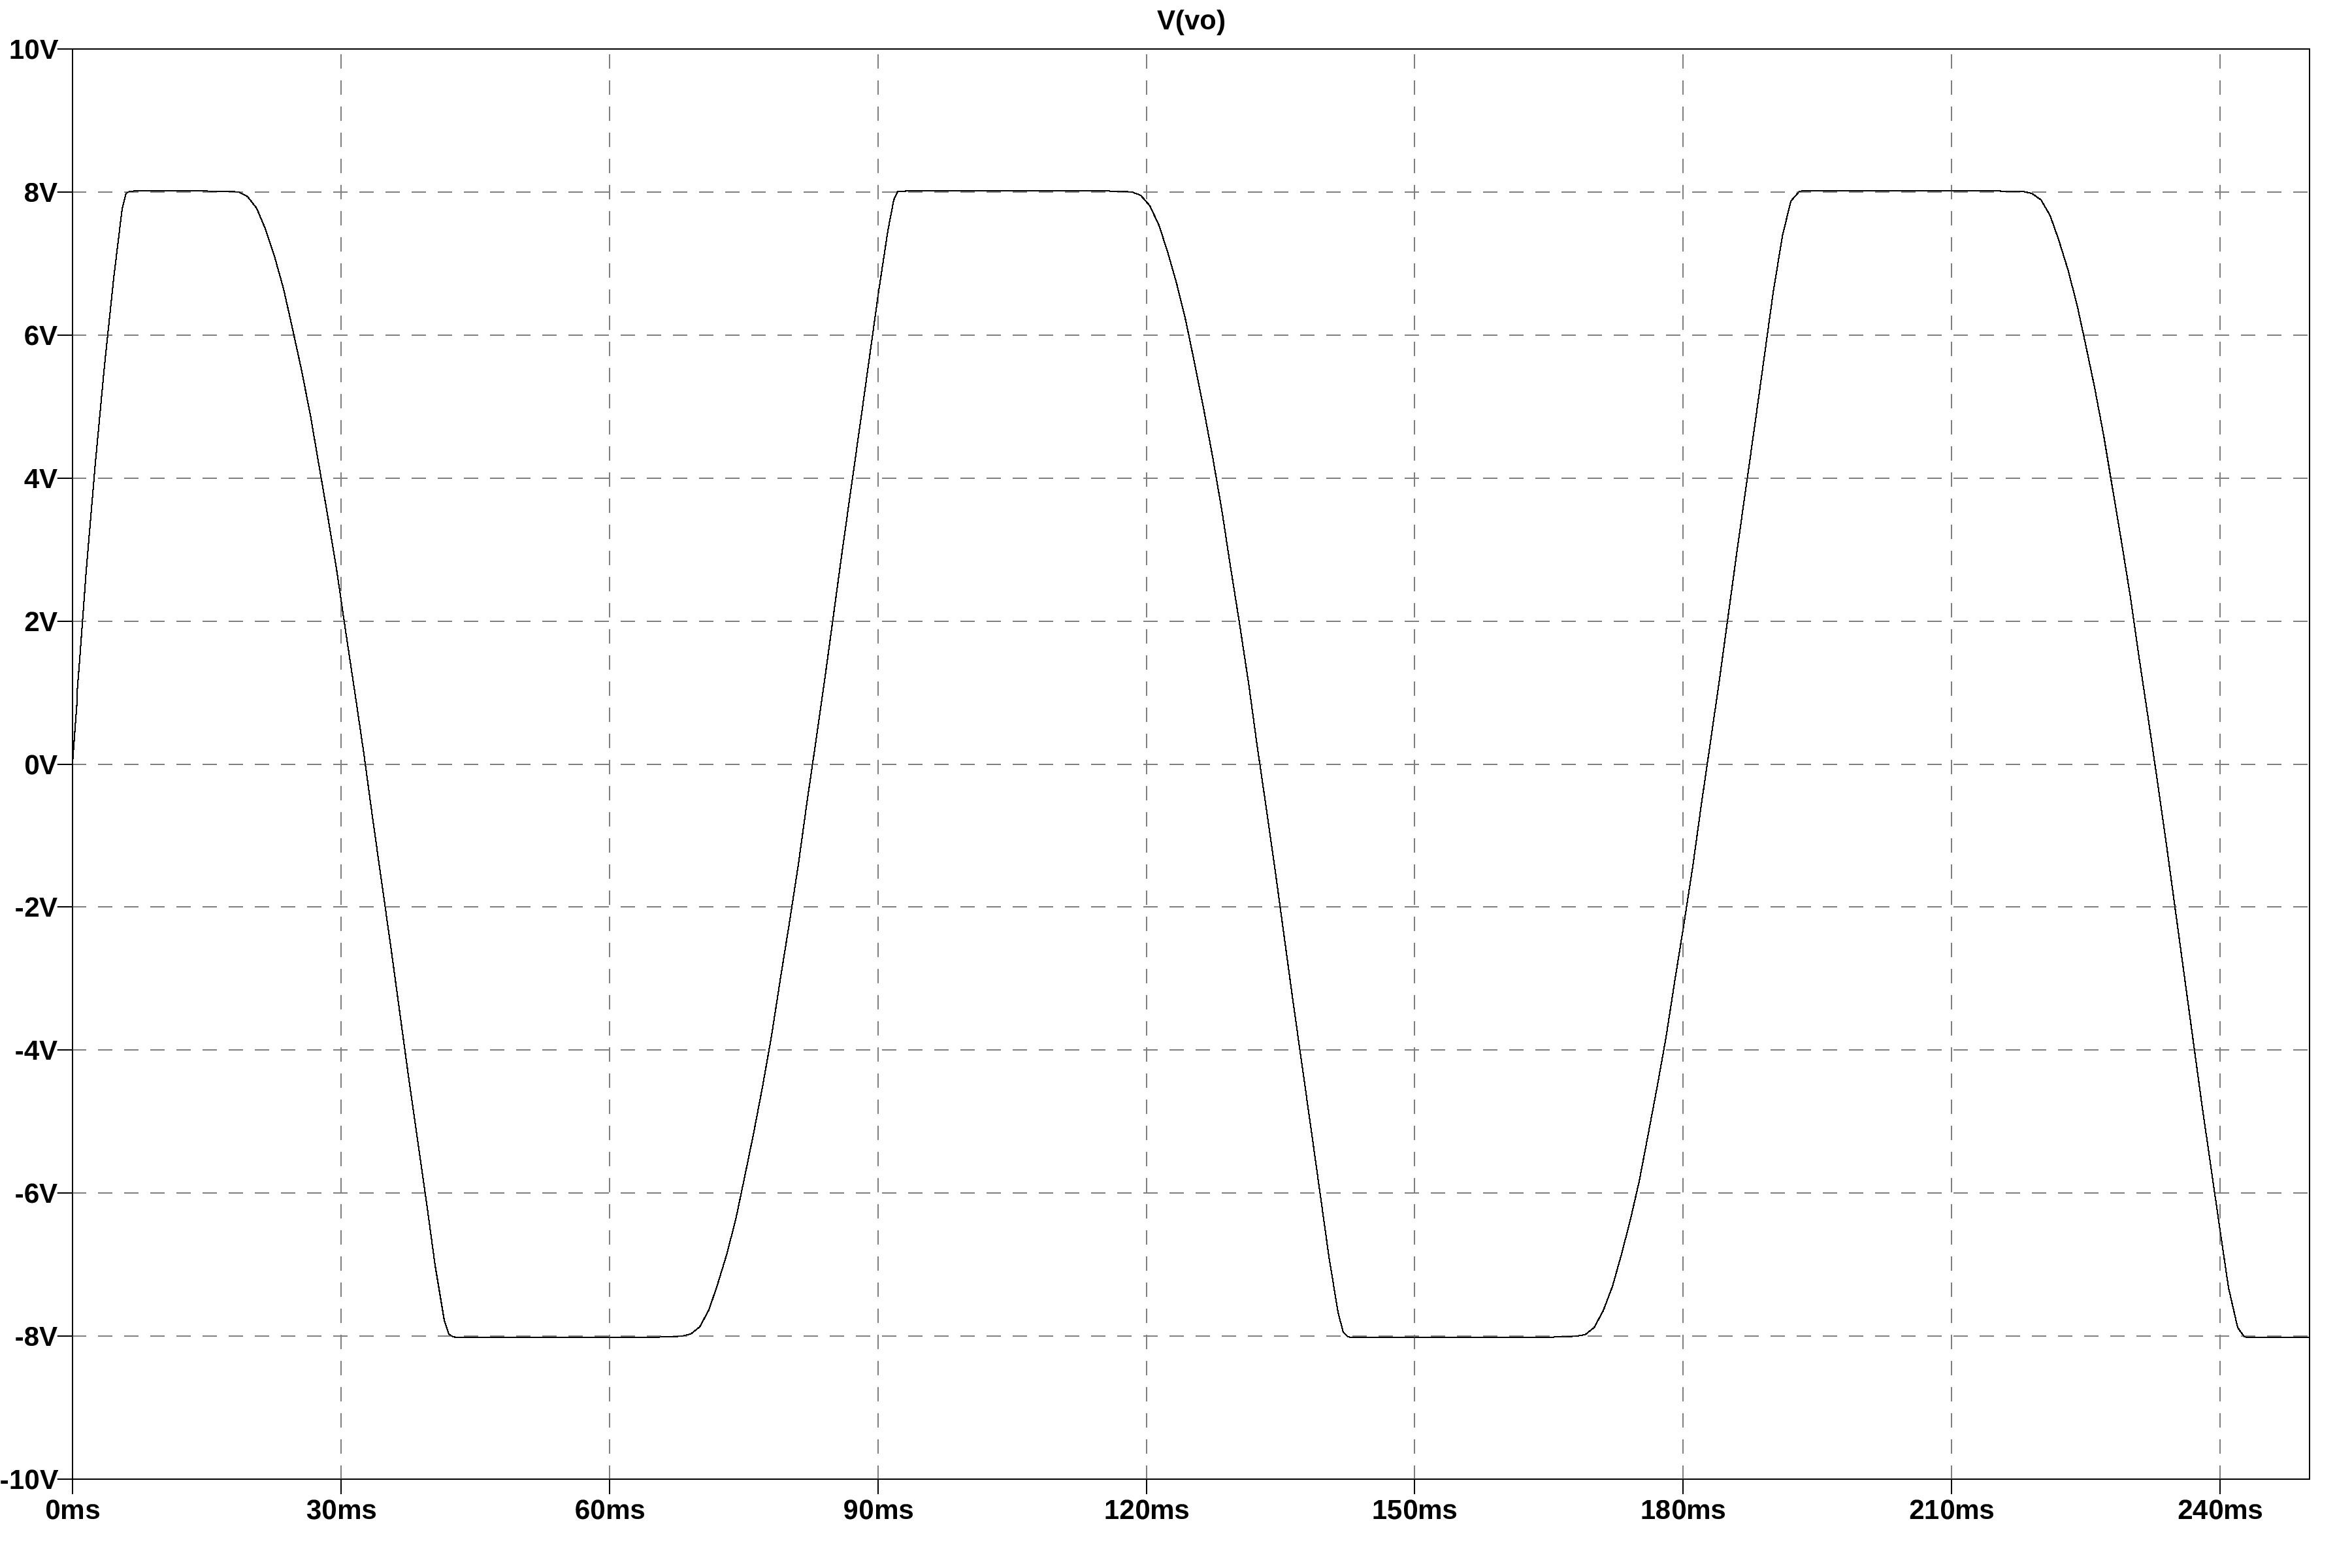
\includegraphics[width=14cm]{graph/1d4c.jpg}
  \caption{Audio Amplifier - Output voltage with an amplitude of the imput voltage equal to $2 \cdot 1.36701V$, frequency equal to $10Hz$}
  \label{1d4cgraph}
\end{figure}

The graph generated is presented on the figure \ref{1d4cgraph}.\\

\subsection{Saturation - LT1028 op. amp. - $R_2 = 109775.2\Omega$}
Using the equation \ref{eq:V_inSat} and setting $\omega = 10Hz \cdot 2\pi$ the maximum value of the input voltage is $|V_{in}| \leq 1.28091V$ (output voltage graph on figure \ref{1d5graph})

\begin{figure}[H]
  \centering
  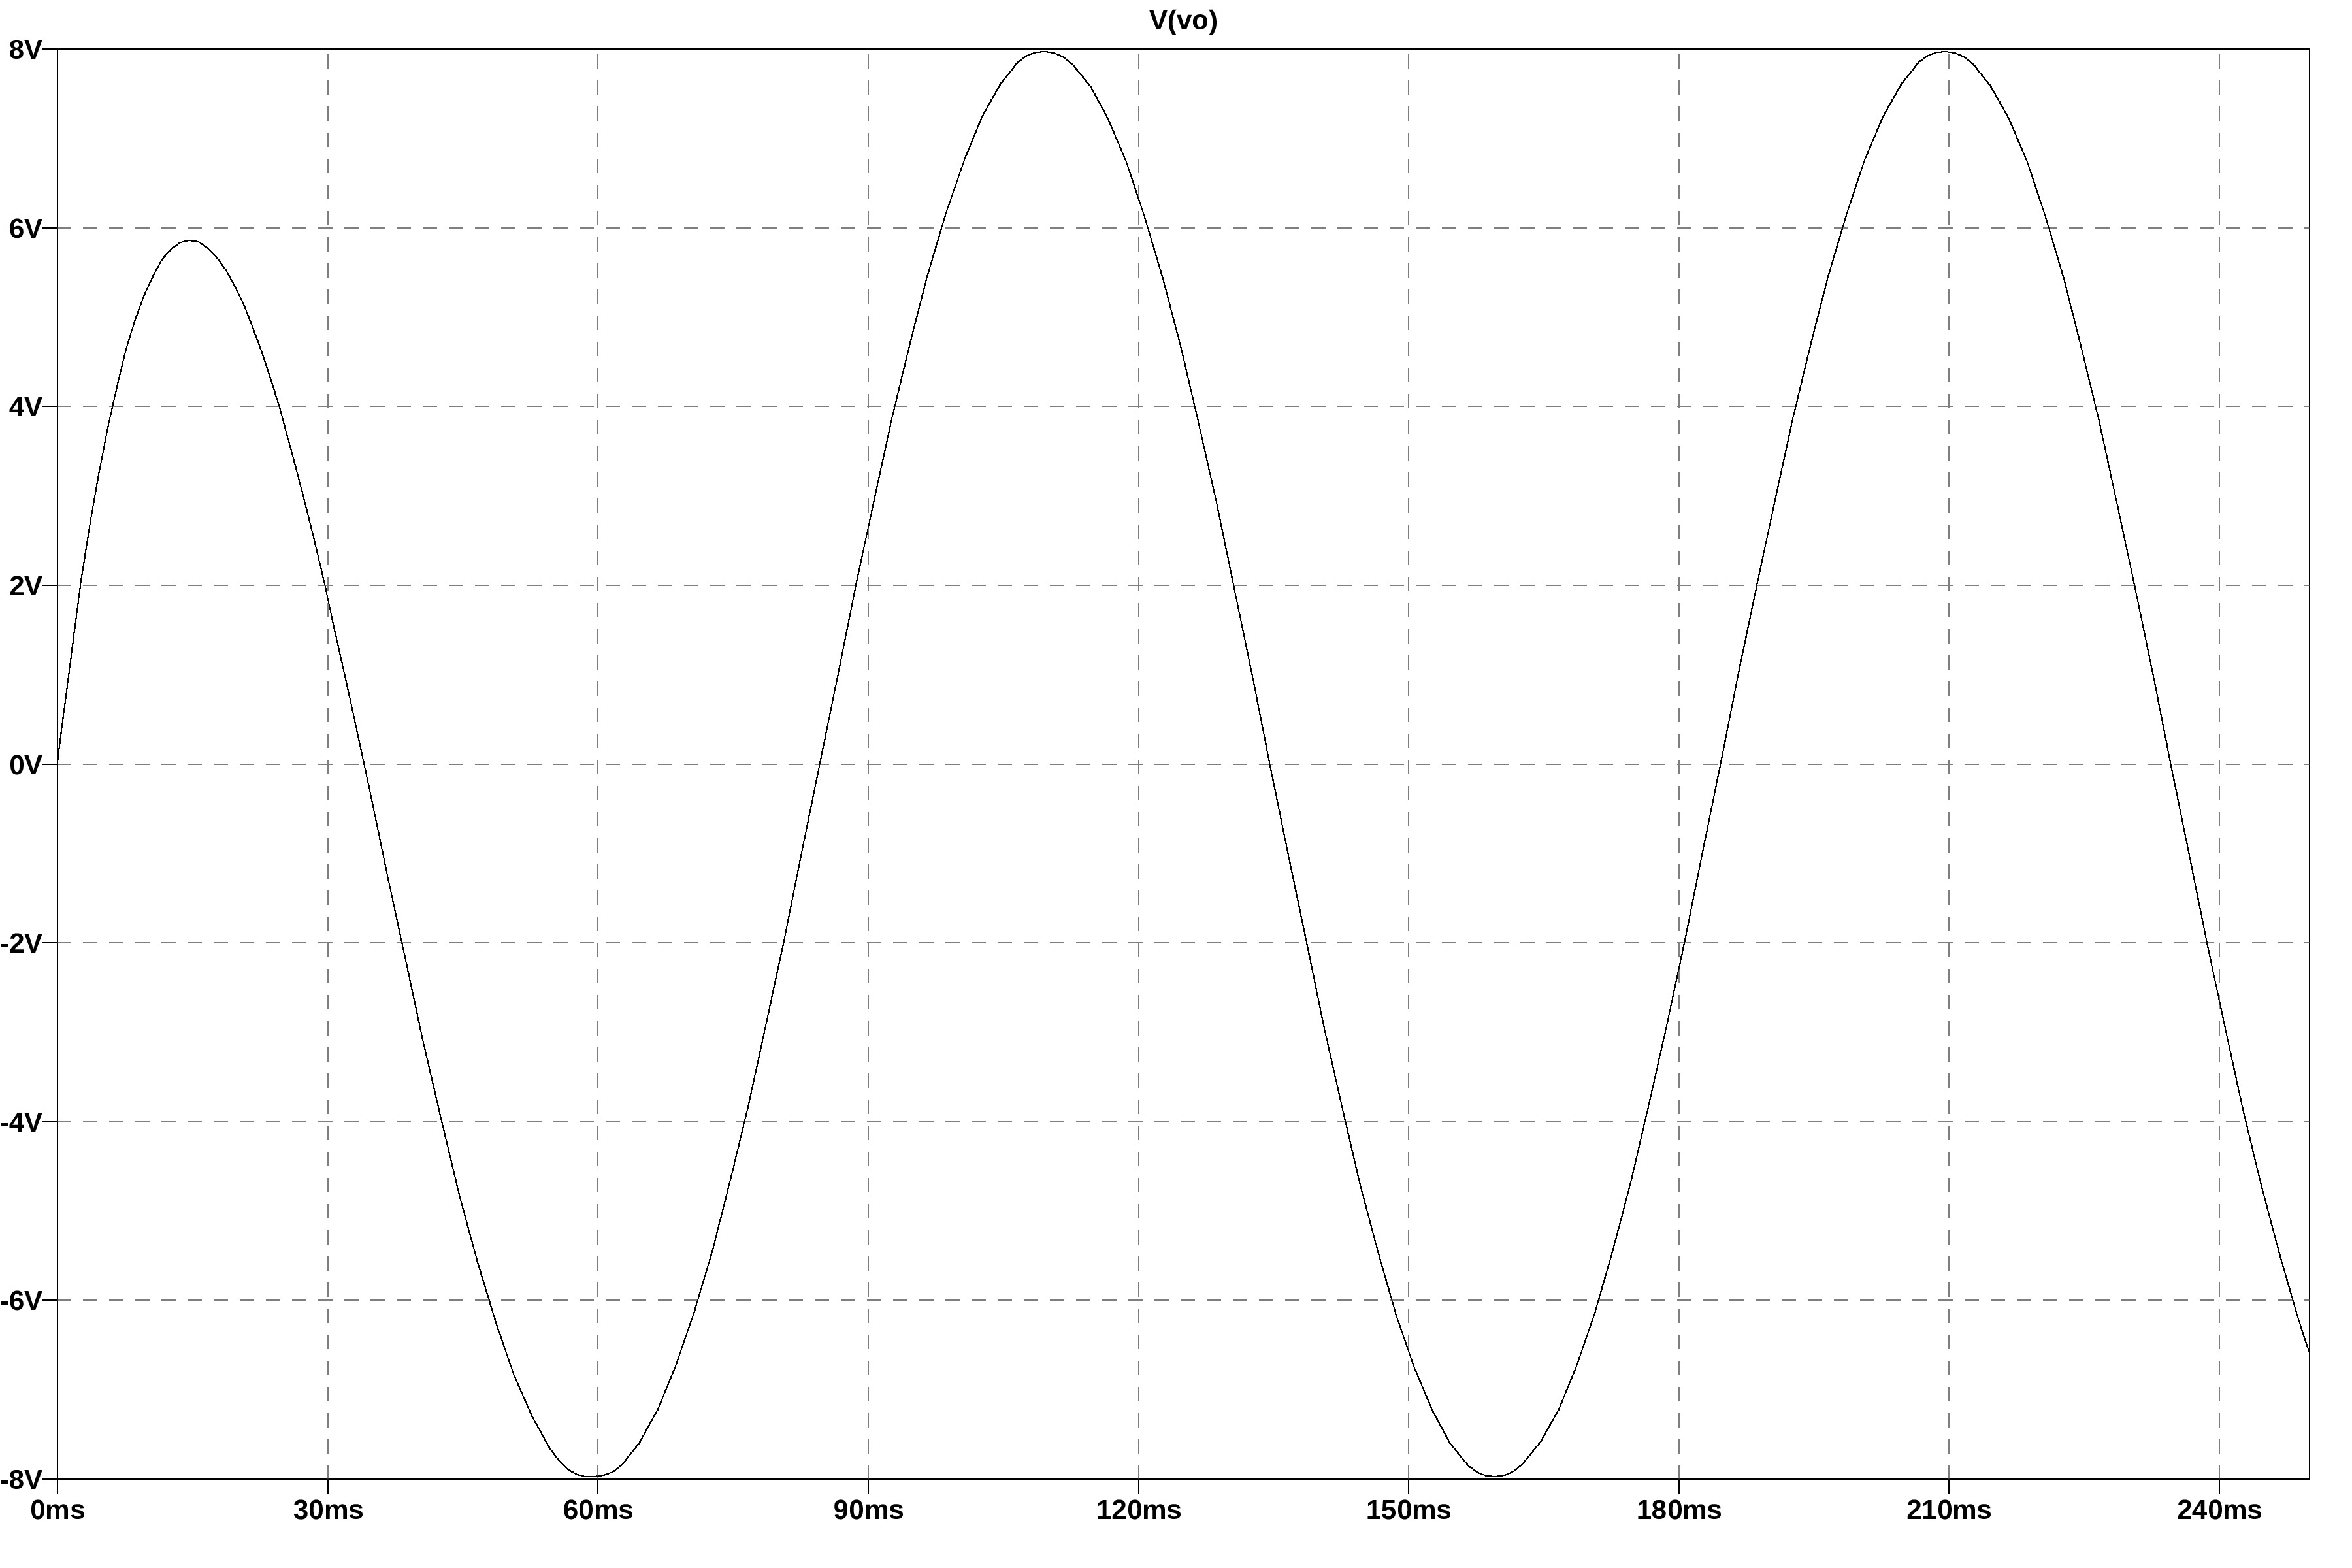
\includegraphics[width=14cm]{graph/1d5.jpg}
  \caption{Audio Amplifier - Output voltage with an amplitude of the imput voltage equal to $1.28091V$, frequency equal to $10Hz$, $R_2$ equal to $109775.2\Omega$}
  \label{1d5graph}
\end{figure}

\subsubsection{Output voltage waveform - $R_2 = 109775.2\Omega$ - $V_{in} = 2 \cdot |V_{in MAX} |$}
The netlist used for plot the output voltage waveform with a double input voltage relatively to the maximum input voltage calculated is:\\
\lstinputlisting{netlist/1d5b.cir}

\begin{figure}[H]
  \centering
  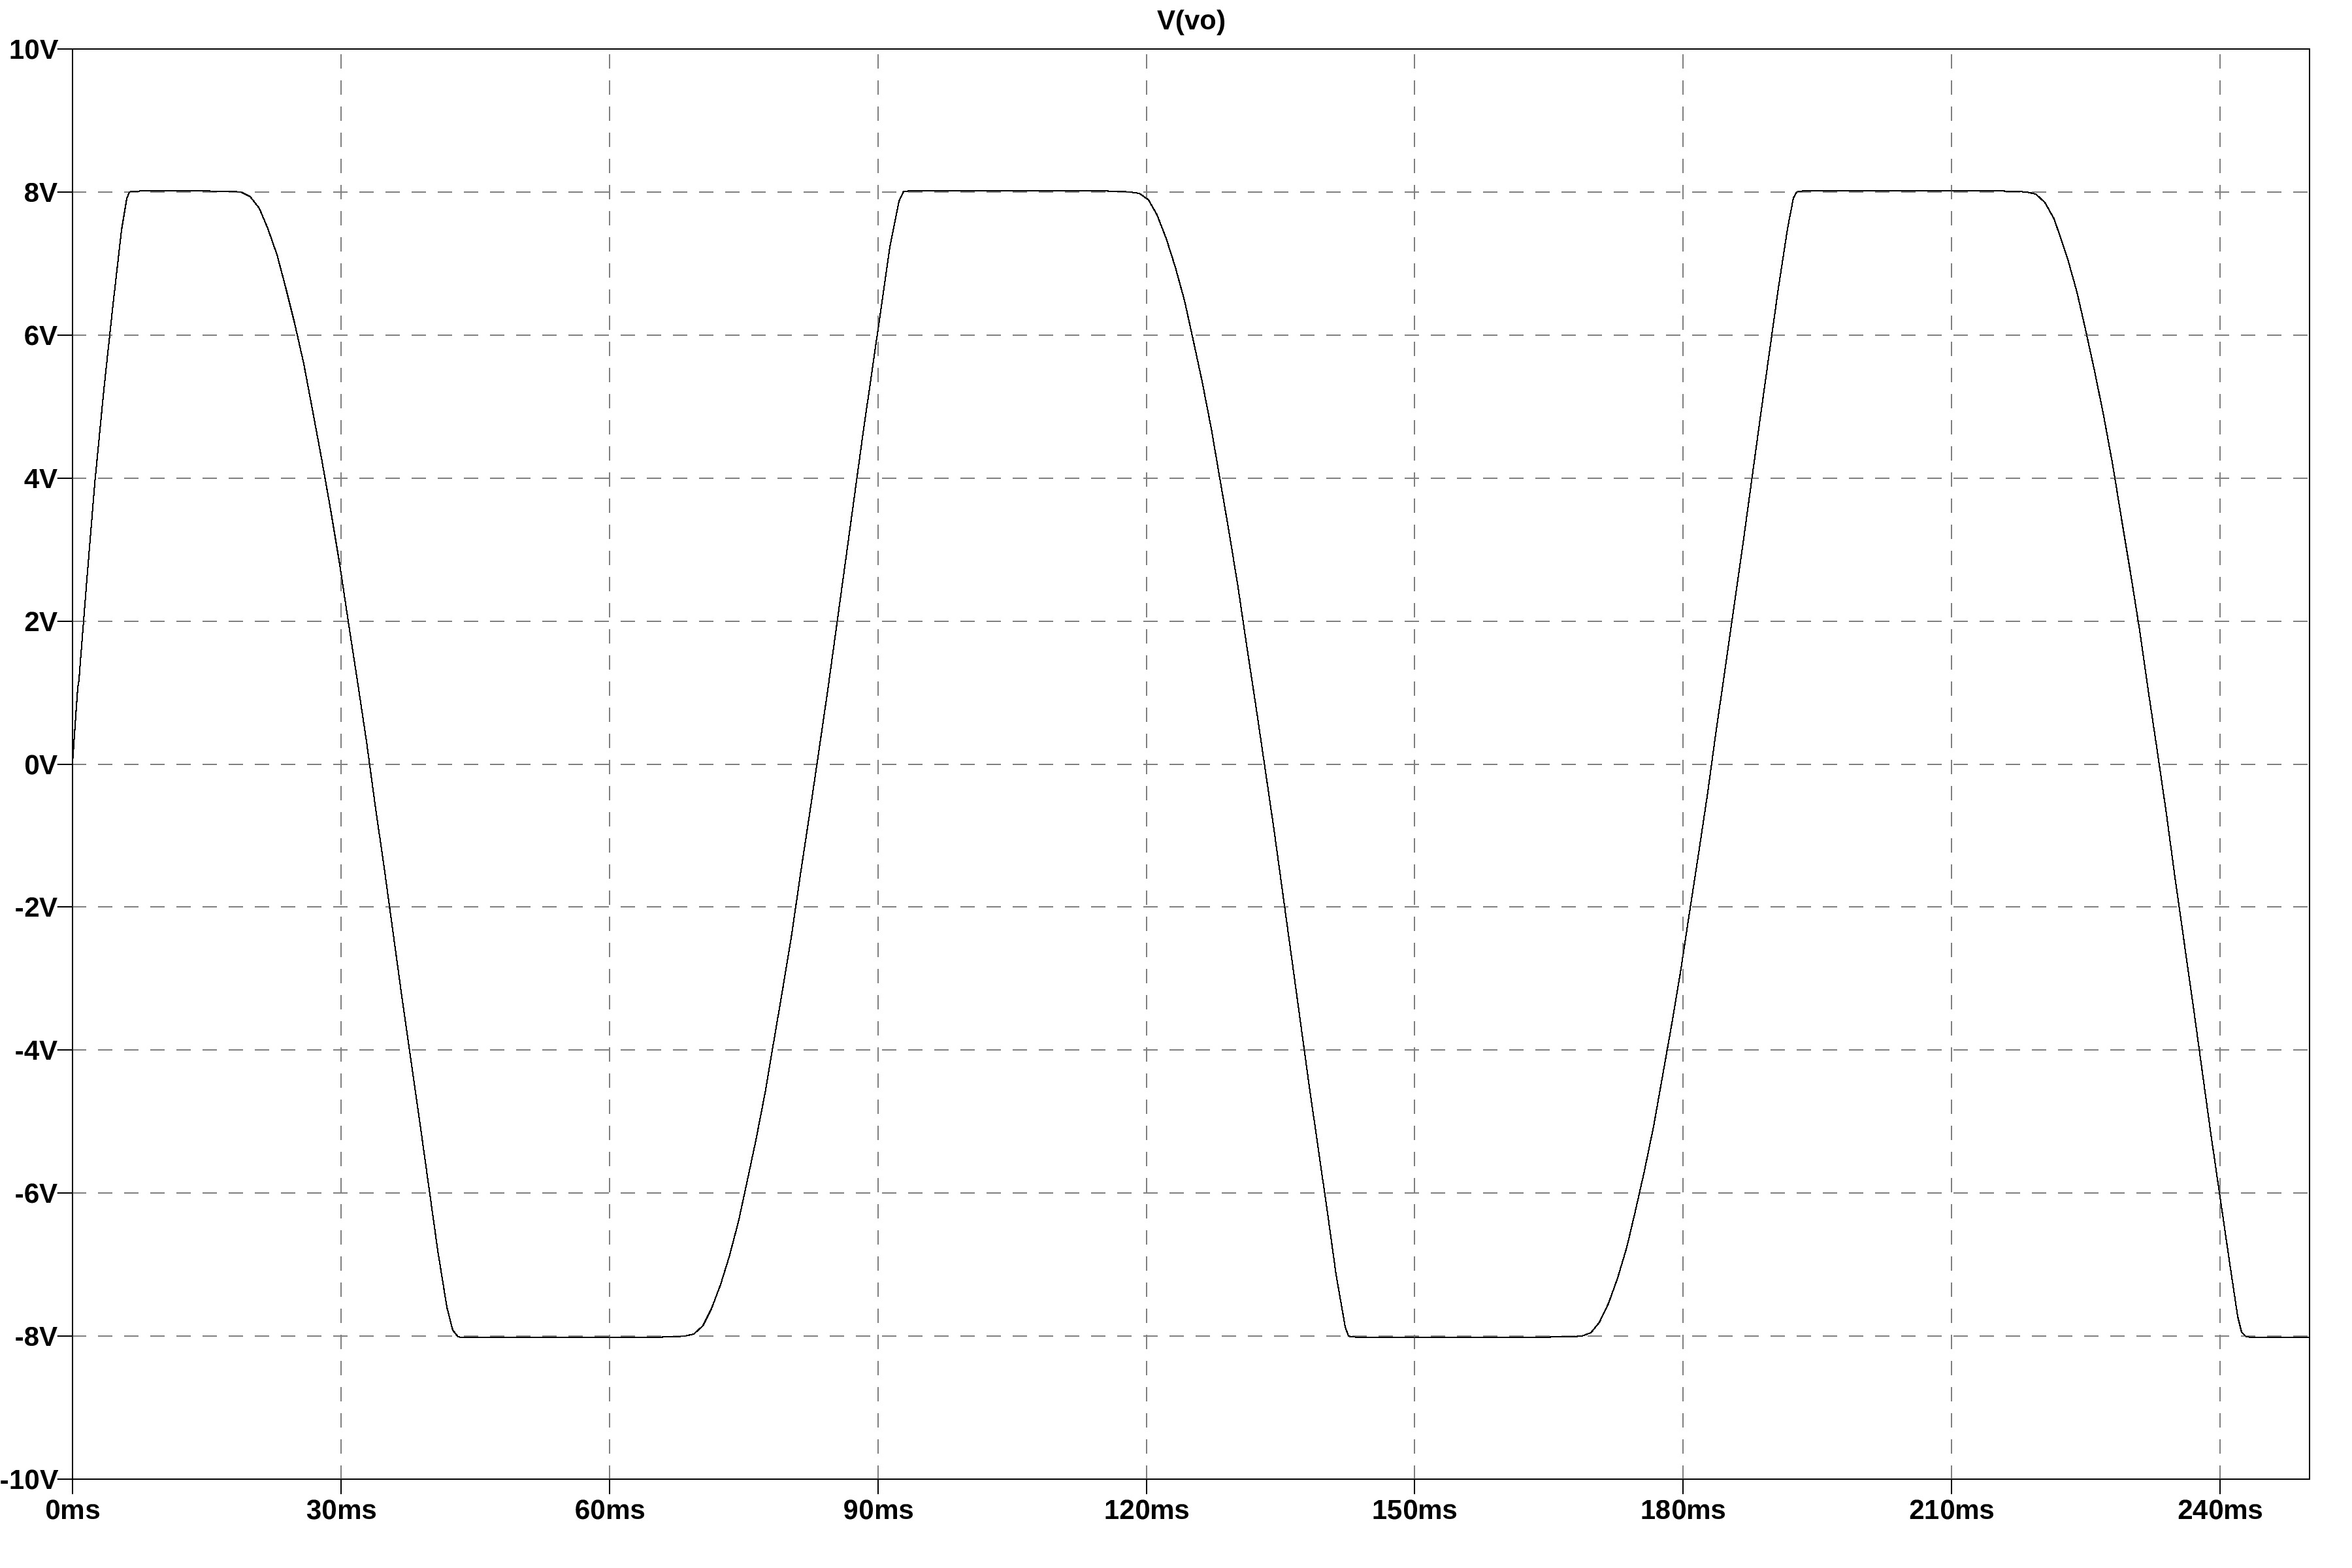
\includegraphics[width=14cm]{graph/1d5b.jpg}
  \caption{Audio Amplifier - Output voltage with an amplitude of the imput voltage equal to $2 \cdot 1.28091V$, frequency equal to $10Hz$, $R_2$ equal to $109775.2\Omega$}
  \label{1d5bgraph}
\end{figure}

The graph generated is presented on the figure \ref{1d5bgraph}.\\

\subsection{Power delivered to the amplifier}

\begin{equation}
P_{DC} = V_{dd} \cdot I_{dd} + V_{ss} \cdot I_{ss}
\end{equation}

\subsubsection{Case A - $R_2 = 100k\Omega$ $V_{in} = 2 \cdot 1.36701V$}
\lstinputlisting{netlist/1d6.cir}

$$P_{DC} = 10V \cdot (-0.00736621A) + (-10V) \cdot (+0.00736621 A) = -0.14732420W$$

\subsubsection{Case B - $R_2 = 109775.2\Omega$ $V_{in} = 2 \cdot 1.28091V$}
\lstinputlisting{netlist/1d6b.cir}

$$P_{DC} = 10V \cdot (-0.00736621A) + (-10V) \cdot (+0.00736621 A) = -0.14732420W$$

\end{document}
